% Provenance (never printed): see sources/outline_sources.md (Year 1: grain size and sorting;
% bedforms and sedimentary structures; fluvial, deltaic, shoreline and deep-sea deposits).
% Exercise and problem values in the Book 3 scratch calculator calc/ch21.py; figure data
% from figdata/bachelor-1/grain_size.py. Meander and delta are Book 1's (g5), sediment and
% sedimentary layer Book 1's (g7), beach Book 1's (g9); the loads, settling, the threshold
% of motion and the Hjulstrom diagram are ch. 20's; the vector mean is ch. 6's. Facies
% models and Walther's law belong to the Year 3 volume (prose pointer only). Pelagic
% sediments are ch. 22's.
\chapter{碎屑沉积及其环境}\label{ch:b1:clastic-sediments}

在海滩上抓起一把沙子，让它从指缝间流下：
颗粒大小几乎一致，磨圆良好、洁净，流动起来像水一样。
在离此数百千米的内陆，古冰川遗留的丘陵脚下，
地面却是由漂石、卵石、沙和泥混成的坚硬混合物，
杂乱无章。两者都由同类碎屑组成，源于同类岩石的破碎，
真正区别二者的，是颗粒的搬运方式与停积之处。
波浪一天往复冲刷数千次，按粒径\omterm{def:b1:clastic-sediments:sorting}{分选}颗粒，
把细颗粒带走并磨圆其余颗粒；
冰川将所拾取的一切全部裹挟，
融化时再一并卸下。本章学习从颗粒本身读出这类“故事”，
从它们在河床和海底所形成的构造，以及
沉积层的叠置顺序中读取这些信息。

\begin{recall}
沉积物是由水、风或冰搬运堆积的松散物质，随时间推移，
沉积物层层堆积，硬结为沉积岩（第~1 册，六年级
和七年级）。沿河漫滩左右摆动的河流形成曲流；河流
注入海洋或湖泊并沉积其载荷时，便形成三角洲；
波浪把沙堆积成海滩，并使其沿岸
漂移（第~1 册，五年级和九年级）。河流以\omterm{def:b1:erosion-transport:load}{推移质}、\omterm{def:b1:erosion-transport:load}{悬移质}
和\omterm{def:b1:erosion-transport:load}{溶解质}的形式搬运载荷；颗粒以\omterm{def:b1:erosion-transport:settling}{沉降速度}下沉；
\omterm{def:b1:erosion-transport:bed-shear}{床面剪应力}超过\omterm{def:b1:erosion-transport:threshold}{起动阈值}时，颗粒开始运动，
\omterm{def:b1:erosion-transport:hjulstrom}{尤尔斯特伦图}给出侵蚀、搬运和沉积的平均速度，
随粒径变化的关系（见\cref{ch:b1:erosion-transport}）。一组方向的矢量平均
为其单位矢量之和的方向，
（见\cref{def:b1:field-lab-methods-1:mean-orientation}）。
\end{recall}

\section{粒度与分选}\label{sec:b1:clastic-sediments:grain-size}

地质学家在记录碎屑沉积物时，首先记录的是颗粒大小，
即由较老岩石碎屑构成的沉积物，因为颗粒大小反映了
沉积它们的水流能量。自然界中颗粒粒径跨越超过七个
数量级，从直径数米的漂石到宽仅千分之一毫米的黏土颗粒，
并以比值标尺进行度量。

\begin{definition}[粒度标尺，phi 标度]\label{def:b1:clastic-sediments:grain-size}
沉积学中的\emph{粒度标尺}\index{粒度标尺}把颗粒直径
分为若干等级，等级界限逐级加倍，
起点为 \qty{1}{mm}；每一等级都有名称（沙、粉砂\ldots）。
\emph{phi 标度}\index{phi 标度}以下式表示直径 $d$：
\[
  \varphi = -\log_2 \frac{d}{\qty{1}{mm}},
\]
于是 $d = 2^{-\varphi}$~mm：\qty{1}{mm} 对应 $\varphi = 0$，\qty{2}{mm} 对应
$\varphi = -1$，\qty{0.25}{mm} 对应 $\varphi = 2$，颗粒越细，
$\varphi$ 值越大。
\end{definition}
% ledger: folk:udden-krumbein, folk:wentworth-classes, usgs:wentworth-phi

在 \omterm{def:b1:clastic-sediments:grain-size}{phi 标度}上，\omterm{def:b1:clastic-sediments:grain-size}{粒度标尺}的每个等级宽度都是一个单位：
从 $d$ 到 $2d$ 的一个等级，对应 $\varphi$ 到 $\varphi - 1$。主要等级
及其常用名称列于\cref{tab:b1:clastic-sediments:classes}中。

\begin{table}[htbp]
\centering\small
\begin{tabular}{@{}lll@{}}
\hline
等级 & 直径（\si{mm}） & $\varphi$ \\
\hline
漂石 & 256 以上 & $-8$ 以下 \\
块石 & 64 至 256 & $-6$ 至 $-8$ \\
卵石 & 4 至 64 & $-2$ 至 $-6$ \\
细砾 & 2 至 4 & $-1$ 至 $-2$ \\
沙（极粗、粗、中、细、极细） & $1/16$ 至 2 & 4 至 $-1$ \\
粉砂（粗、中、细、极细） & $1/256$ 至 $1/16$ & 8 至 4 \\
黏土 & $1/256$ 以下（\qty{3.9}{\micro m}） & 8 以上 \\
\hline
\end{tabular}
\caption{粒度等级。沙的五个等级各为
phi 单位宽，由极粗（1 至 \qty{2}{mm}）到极细（$1/16$ 至
$1/8$~mm）；粉砂的四个等级亦然。部分学者将粉砂的
下限定为 9，而非 $8\,\varphi$。砾石是泛指
粗于 \qty{2}{mm} 的颗粒的统称，泥则指粉砂与黏土的混合物。}
\label{tab:b1:clastic-sediments:classes}
\end{table}
% ledger: folk:wentworth-classes, usgs:wentworth-phi

\emph{黏土}一词在本书中有两种含义：此处指一种粒级，
在\cref{ch:b1:weathering-clays}中则指一类\omterm{def:b1:rock-forming-minerals:mineral}{矿物}。多数黏土粒级的颗粒
是\omterm{def:b1:weathering-clays:clay-mineral}{黏土矿物}，多数\omterm{def:b1:weathering-clays:clay-mineral}{黏土矿物}也属黏土粒级，但二者并不完全重合：
磨得极细的石英属于黏土粒级，\omterm{def:b1:weathering-clays:clay-mineral}{高岭石}片晶
则可以达到粉砂的大小。

\emph{粒径的测量。}砾石逐粒用卡尺测量。
沙用筛分法测定：一套网孔按每整数或半个 phi 单位
递变的筛子经振摇后，称量各筛上的截留量。粉砂与黏土比
$4\,\varphi$ 更细，用沉降法测定：将沉积物搅入水中，
由于每个颗粒的下沉速度由其大小决定（斯托克斯定律，
见\cref{prop:b1:erosion-transport:stokes}），则某一深度与时刻仍悬浮的质量
可说明样品中细于某一给定
直径的部分有多少。测量颗粒光散射的激光仪器现在也很常用，
结果是各等级质量百分比的列表。

\begin{definition}[平均粒径，分选]\label{def:b1:clastic-sediments:sorting}
设沉积物的粒径以 phi 为单位，其分布由
各等级的质量给出。其\emph{平均粒径}\index{平均粒径}是
该分布的均值，其\emph{分选}\index{分选}为该分布的
离散程度，以 phi 为单位的标准差度量：
沉积物在颗粒几乎全部为同一粒径时分选良好，
颗粒跨越多个等级时分选较差。两者可由
各等级的百分含量用矩法计算，或由
累积曲线按福克的图解度量计算：
\[
  M_z = \frac{\varphi_{16} + \varphi_{50} + \varphi_{84}}{3}, \qquad
  \sigma_I = \frac{\varphi_{84} - \varphi_{16}}{4} + \frac{\varphi_{95} - \varphi_{5}}{6.6},
\]
其中 $\varphi_p$ 是以 phi 为单位的粒径，样品中
有 $p$% 比其更粗。
\end{definition}
% ledger: folk:graphic-measures

\begin{method}[由筛分分析求平均值与分选]\label{met:b1:clastic-sediments:graphic}
\begin{enumerate}
  \item 按粒级由粗到细列出各粒级的重量百分比 $w_i$，
        并检查其总和是否为 \qty{100}{\percent}（或以之相除）。
  \item \emph{矩法。}设 $x_i$ 为第 $i$ 粒级的中点（以 phi 为单位），
        则计算平均值 $m = \sum w_i x_i / 100$ 和标准差
        $s = \sqrt{\sum w_i (x_i - m)^2 / 100}$。
  \item \emph{图解度量。}累计各百分比，求得比各粒级界限更粗的
        重量百分比，并以之对 $\varphi$ 作图：
        即累积曲线。
  \item 在累积曲线上，由粒级界限之间的线性插值读出粒径
        $\varphi_5$、$\varphi_{16}$、$\varphi_{50}$、$\varphi_{84}$ 和
        $\varphi_{95}$。
  \item 计算 $M_z$ 与 $\sigma_I$（见\cref{def:b1:clastic-sediments:sorting}），
        将 $M_z$ 按 $d = 2^{-M_z}$ 换算为毫米，
        并依下列标度给出\omterm{def:b1:clastic-sediments:sorting}{分选}等级。
\end{enumerate}
\end{method}

两种方法给出的结果几乎相同，其原因
在于下述性质。

\begin{proposition}[正态分布的图解度量]\label{prop:b1:clastic-sediments:normal}
若沉积物的粒径（以 phi 为单位）服从正态分布，其均值为
$\mu$、标准差为 $\sigma$，则 $M_z = \mu$，$\sigma_I = 0.996\,\sigma$。
\end{proposition}

\begin{proof}
对正态分布而言，数值落在 $\mu + z\sigma$ 以下的比例
仅依赖于 $z$；低于 $\mu + 0.9945\,\sigma$ 的比例为 \qty{84}{\percent}，
低于 $\mu + 1.6449\,\sigma$ 的比例为 \qty{95}{\percent}（正态分布的数值，
在本阶段不加证明地承认）。由对称性，$\varphi_{50} = \mu$，$\varphi_{16} = \mu -
0.9945\,\sigma$，$\varphi_{84} = \mu + 0.9945\,\sigma$，$\varphi_5 = \mu -
1.6449\,\sigma$ 及 $\varphi_{95} = \mu + 1.6449\,\sigma$（百分位数按较粗部分计，
即较小的 $\varphi$，但分布是
对称的）。于是 $M_z = (3\mu)/3 = \mu$，并且
\[
  \sigma_I = \frac{2 \times 0.9945\,\sigma}{4} + \frac{2 \times 1.6449\,\sigma}{6.6}
  = (0.4972 + 0.4985)\,\sigma = 0.996\,\sigma. \qedhere
\]
\end{proof}

福克公式中常数 6.6 正是为此而取：第
5 至第 95 百分位的区间跨越 $3.29$ 个正态分布的
标准差，公式对两个区间给出的 $\sigma$ 估计取平均，
即 $(\varphi_{84}-\varphi_{16})/2$ 与 $(\varphi_{95}-\varphi_5)/3.3$。
同时利用曲线的两端与中部约三分之二，使 $\sigma_I$
对粗粒与细粒混入组分十分敏感，这些组分最能说明沉积物
是如何沉积的。

\begin{omfigure}
\begin{tikzpicture}[font=\small]
% grain-size histograms and cumulative curves of two invented samples (figdata/bachelor-1/grain_size.py)
\begin{axis}[name=a, width=7.3cm, height=6cm, xmin=-5.5, xmax=10.5, ymin=0, ymax=90,
    xlabel={粒径 $\varphi$}, ylabel={各粒级的重量百分比},
    title={\footnotesize (a) 直方图}, xtick={-4,-2,...,10}, ytick={0,20,...,80},
    legend style={at={(0.03,0.97)}, anchor=north west, font=\scriptsize}, legend cell align=left]
  \addplot[ybar interval, fill=omDef!35, draw=omDef, area legend] table[x=phi, y=wt] {figdata/out/bachelor-1-grain_size-step-beach.dat} \closedcycle;
  \addplot[const plot, fill=omThm!20, draw=omThm, fill opacity=0.6, area legend] table[x=phi, y=wt] {figdata/out/bachelor-1-grain_size-step-till.dat} \closedcycle;
  \legend{海滩砂（半 phi 粒级）, 冰碛物（整 phi 粒级）}
\end{axis}
\begin{axis}[at={(a.east)}, anchor=west, xshift=1.6cm, width=7.3cm, height=6cm, xmin=-5.5, xmax=10.5, ymin=0, ymax=100,
    xlabel={粒径 $\varphi$}, ylabel={比该粒径粗的重量百分比},
    title={\footnotesize (b) 累积曲线}, xtick={-4,-2,...,10}, ytick={0,16,50,84,100},
    grid=major, grid style={black!10}]
  \addplot[omDef, very thick, mark=*, mark size=1.2pt] table[x=phi, y=cum] {figdata/out/bachelor-1-grain_size-cum-beach.dat};
  \addplot[omThm, very thick, mark=*, mark size=1.2pt] table[x=phi, y=cum] {figdata/out/bachelor-1-grain_size-cum-till.dat};
  \node[font=\footnotesize, omDef, anchor=west] at (axis cs:2.9,40) {海滩砂};
  \node[font=\footnotesize, omThm, anchor=west] at (axis cs:5.4,72) {冰碛物};
\end{axis}
\end{tikzpicture}

{\small 两种沉积物的粒度分布，取自筛分与沉降
分析（虚构数据）。(a)~各粒级的重量百分比：海滩砂
几乎全部落在三个半 phi 粒级的中砂与细砂之中；
冰碛物分布于十五个 phi 粒级，从卵石到黏土。(b)~累积曲线，
即比各粒径粗的重量百分比：曲线越陡，
\omterm{def:b1:clastic-sediments:sorting}{分选}越好。由 5、16、50、84 和 95 百分位读出的图解度量
给出砂的 $M_z = 2.25\,\varphi$（\qty{0.21}{mm}）与 $\sigma_I =
0.36\,\varphi$；冰碛物的 $M_z = 1.83\,\varphi$ 与 $\sigma_I = 3.84\,\varphi$。}
\label{fig:b1:clastic-sediments:grain-size}
\end{omfigure}
% ledger: folk:graphic-measures

\emph{\omterm{def:b1:clastic-sediments:sorting}{分选}的文字描述。}福克根据大量实测沉积物，提出了
$\sigma_I$ 的文字标度：小于 \num{0.35} 为\omterm{def:b1:clastic-sediments:sorting}{分选}很好，\num{0.35} 至
\num{0.50} 为\omterm{def:b1:clastic-sediments:sorting}{分选}好，\num{0.50} 至 \num{0.71} 为中等偏好，
\num{0.71} 至 \num{1.0} 为中等，\num{1.0} 至 \num{2.0} 为\omterm{def:b1:clastic-sediments:sorting}{分选}差，
\num{2.0} 至 \num{4.0} 为\omterm{def:b1:clastic-sediments:sorting}{分选}很差，大于 \num{4.0} 为\omterm{def:b1:clastic-sediments:sorting}{分选}极
差。天然沉积物所达到的最佳\omterm{def:b1:clastic-sediments:sorting}{分选}约为 \num{0.20} 至
\num{0.25}，他测得的\omterm{def:b1:clastic-sediments:bedform}{沙丘}与海滩砂介于
\num{0.25} 与 \num{0.35} 之间；河流沉积物为 \num{0.40} 至 \num{2.5}，
河漫滩与陆架的粉砂及黏土约为 \num{2.0} 至 \num{3.5}，
\omterm{def:b1:clastic-sediments:sorting}{分选}最差的则是冰碛物与泥流。图中海滩
砂为 \num{0.36}，\omterm{def:b1:clastic-sediments:sorting}{分选}好，接近\omterm{def:b1:clastic-sediments:sorting}{分选}很好的边界；
冰碛物为 \num{3.84}，\omterm{def:b1:clastic-sediments:sorting}{分选}很差。对冰碛物，矩法
给出的平均值为 $1.89\,\varphi$，标准差为
$3.64\,\varphi$，与图解值接近；两者的差异来自
两端及分布的不对称性。
% ledger: folk:sorting-classes, folk:natural-sorting

\omterm{def:b1:clastic-sediments:sorting}{分选}是搬运的记录。水流能\omterm{def:b1:clastic-sediments:sorting}{分选}其载荷，是因为
其能搬动与悬浮的颗粒，取决于各自的粒径
（见\cref{sec:b1:erosion-transport:threshold}）：海滩上的波浪与\omterm{def:b1:clastic-sediments:bedform}{沙丘}上的风
反复作用于同样的颗粒，带走细粒，留下
过重而难以搬动的颗粒，其沉积物\omterm{def:b1:clastic-sediments:sorting}{分选}在所有沉积中最好。
冰川、碎屑流以及洪水的骤然倾泻都不\omterm{def:b1:clastic-sediments:sorting}{分选}。

\emph{形状与圆度。}颗粒的圆度描述其棱角的锐利程度，
与其整体形状无关：瓦德尔将其定义为棱角处的平均曲率半径，
除以最\omterm{def:b1:spherical-astronomy:spherical-triangle}{大圆}的半径，该圆能内切于颗粒轮廓，
其值从球体的 1 降至
碎片的接近 0。测量它十分繁琐，故改用照片图表比较颗粒；
在瓦德尔标度上，大多数砂粒的圆度为
\num{0.3} 至 \num{0.4}；在福克的对数标度上，由 0（很尖棱角状）
至 6（很圆），约为 \num{2.5}，属次棱角状。对砂粒而言，磨圆很慢：
风吹石英的磨圆远快于水中搬运的石英，水
能缓冲撞击；海滩砂磨圆比河砂快，而砂粒在河流中
几乎得不到磨圆。卵石在河流中磨圆很快，软者先
磨圆：在科罗拉多河上，石灰岩卵石达到最终的
圆度只需几英里之内，而石英卵石约需 150 英里才能赶上。
% ledger: folk:roundness, folk:rounding

\begin{definition}[结构成熟度，成分成熟度]\label{def:b1:clastic-sediments:maturity}
一片砂或砂岩的\emph{结构成熟度}\index{结构成熟度}，
度量水流的\omterm{def:b1:clastic-sediments:sorting}{分选}、磨蚀与淘洗作用对其改造的程度，分为四个阶段：
\emph{未成熟}，泥质杂基含量超过
\qty{5}{\percent}；\emph{次成熟}，泥质较少，但\omterm{def:b1:clastic-sediments:sorting}{分选}差
（$\sigma > 0.5\,\varphi$）；\emph{成熟}，泥质很少或不含，
\omterm{def:b1:clastic-sediments:sorting}{分选}好（$\sigma < 0.5\,\varphi$），但颗粒呈棱角状；
\emph{超成熟}，不含泥质，颗粒既\omterm{def:b1:clastic-sediments:sorting}{分选}好又磨圆好。
其\emph{成分成熟度}\index{成分成熟度}，度量
不稳定\omterm{def:b1:rock-forming-minerals:mineral}{矿物}与岩屑被去除、只剩石英的程度：
在几乎纯石英的砂岩中很高，在富含\omterm{def:b1:rock-forming-minerals:groups}{长石}、
\omterm{def:b1:rock-forming-minerals:groups}{云母}或岩屑的砂岩中很低。
\end{definition}
% ledger: folk:maturity, folk:mineral-maturity

\omterm{def:b1:clastic-sediments:maturity}{结构成熟度}应从沉积物沉积时的状况来读取：
晚期在孔隙中结晶的\omterm{def:b1:weathering-clays:clay-mineral}{黏土矿物}，
以及把颗粒胶结在一起的胶结物（见\cref{ch:b1:diagenesis-basins}），
都不计入。它反映沉积地点的能量：未成熟的沉积物
堆积在河漫滩、冲积扇和泻湖中，那里水流微弱，
或沉积过快，以致颗粒来不及被改造；超成熟的沉积物
则形成于海滩与沙漠\omterm{def:b1:clastic-sediments:bedform}{沙丘}，那里能量无休止地作用于颗粒。
\omterm{def:b1:clastic-sediments:maturity}{成分成熟度}由磨蚀与风化共同决定。\omterm{def:b1:rock-forming-minerals:groups}{长石}比石英软，
且具良好的解理，被磨蚀得更快；棱角状石英与同粒径\omterm{def:b1:rock-forming-minerals:groups}{长石}
组成的\omterm{def:b1:rock-forming-minerals:groups}{长石}砂岩，仅靠磨蚀，就可能变为超成熟砂岩，
其中的砂几乎全是石英，\omterm{def:b1:rock-forming-minerals:groups}{长石}只以粉砂的形式残留。
风化作用发生在物源区及沿途长期堆存的过程中，
同样通过把\omterm{def:b1:rock-forming-minerals:groups}{长石}变为黏土起作用
（见\cref{sec:b1:weathering-clays:hydrolysis}）。
形成于\omterm{def:b1:layered-earth:layers}{地壳}动荡时期、又从隆起山脉迅速侵蚀而来的砂岩，
两种意义上通常都未成熟；形成于平静时期、长期被再改造的砂岩，
往往是超成熟的石英砂岩；但例外很多，任何成分都可以出现在任一阶段的\omterm{def:b1:clastic-sediments:maturity}{结构成熟度}中。
% ledger: folk:maturity, folk:mineral-maturity

\section{床形与沉积构造}\label{sec:b1:clastic-sediments:bedforms}

水流裹挟砂粒越过床面时，床面很少保持平坦，
而是自行组织成随水流移动的砂波。这些形态，
以及它们在沉积物内部留下的层理，
是过去水流最直接的记录。

\begin{definition}[床形，波痕，沙丘]\label{def:b1:clastic-sediments:bedform}
\emph{床形}\index{床形}是水流在松散颗粒床面上塑造出的规则起伏，
沿水流方向重复出现。\emph{波痕}\index{波痕}是一种小型床形，
高数厘米，相邻波峰间距为 10 至 \qty{20}{cm}，迎流一侧（迎流面）平缓，
背流一侧（背流面）陡峭；\emph{沙丘}\index{沙丘}形状相似，
但至少大十倍，
水下高度从分米到米不等。
\end{definition}
% ledger: southard:ripples-dunes

\omterm{def:b1:clastic-sediments:bedform}{波痕}的迎流面坡度小于约 \ang{10}；其背流一侧，即
滑落面，接近砂在水中的休止角，约为 \ang{30}。
砂粒从迎流面被侵蚀，越过波峰，沿背流面崩落或洒落，
于是整个\omterm{def:b1:clastic-sediments:bedform}{波痕}顺流移动，速度远慢于水流，
方式是从其后部取走颗粒、加到前部。
风在陆地上也形成同类的\omterm{def:b1:clastic-sediments:bedform}{波痕}与\omterm{def:b1:clastic-sediments:bedform}{沙丘}，沙漠中的\omterm{def:b1:clastic-sediments:bedform}{沙丘}
远大于河流中的\omterm{def:b1:clastic-sediments:bedform}{沙丘}。
% ledger: southard:ripples-dunes, southard:climb

\begin{proposition}[床形迁移与推移质]\label{prop:b1:clastic-sediments:migration}
一列剖面为三角形、高为 $H$ 的\omterm{def:b1:clastic-sediments:bedform}{床形}，以速度 $c$ 顺流移动、形状不变，
其迎流面被侵蚀、背流面发生沉积，
每单位宽度、单位时间越过波峰的
\omterm{def:b1:erosion-transport:load}{推移质}体积为
\[
  q_b = (1 - p)\,\frac{c\,H}{2},
\]
以固体颗粒计，其中 $p$ 为砂的孔隙度。
\end{proposition}

\begin{proof}
在固定点上跟踪床面，观察一个\omterm{def:b1:clastic-sediments:bedform}{床形}经过所用的时间为 $L/c$，其中 $L$
为其长度。\omterm{def:b1:clastic-sediments:bedform}{床形}中位于槽线以上的每个颗粒，都已越过
其后方\omterm{def:b1:clastic-sediments:bedform}{床形}的波峰，因为\omterm{def:b1:clastic-sediments:bedform}{床形}只通过
颗粒从迎流面转移到背流面而移动。\omterm{def:b1:clastic-sediments:bedform}{床形}的截面积为 $LH/2$，
即底为 $L$、高为 $H$ 的三角形，其中颗粒占比为 $1 - p$。
这部分颗粒体积在时间 $L/c$ 内越过每个波峰，因此通量为
$(1-p)(LH/2)/(L/c) = (1-p)cH/2$。未在背流面沉积、直接越过\omterm{def:b1:clastic-sediments:bedform}{床形}的
那部分负荷不计入，因此该公式给出的
是\omterm{def:b1:erosion-transport:load}{推移质}的下界。
\end{proof}

\emph{床面相的序列。}在床面为中粒砂的实验室水槽中，
流速逐渐增大时，床面依次形成一组固定的构型。
低于\omterm{def:b1:erosion-transport:threshold}{起动阈值}时，床面保持平坦；刚超过阈值时出现\omterm{def:b1:clastic-sediments:bedform}{波痕}；
约为每秒零点几米的流速时，它们
在仅差数厘米每秒的流速范围内被\omterm{def:b1:clastic-sediments:bedform}{沙丘}取代。流速更快时，\omterm{def:b1:clastic-sediments:bedform}{沙丘}
被压平，床面重新变为平面，即上平床，砂在其上
以致密的砂层和悬浮方式移动。最后，当平均流速 $U$
接近表面波在水中的速度 $\sqrt{gh}$（水深为 $h$）时，即
弗劳德数 $U/\sqrt{gh}$ 趋近于 1 时，水面与床面
形成同相位的波动，波动增长、变陡、破碎并再次形成，称为反\omterm{def:b1:clastic-sediments:bedform}{沙丘}，
由吉尔伯特在 1914 年的水槽实验中命名，因其波峰向上游移动。
反\omterm{def:b1:clastic-sediments:bedform}{沙丘}需要浅而快的水流，在
深度超过数米的水流中并不重要。
% ledger: southard:ripples-dunes

粒径会改变这一序列。\omterm{def:b1:clastic-sediments:bedform}{波痕}只在细于约 \qty{0.8}{mm} 的砂中形成；
在粗砂与砾石中，床面由无运动的平床，
先变为颗粒运动的低平床，再直接转为\omterm{def:b1:clastic-sediments:bedform}{沙丘}。
在细砂（约 \qty{0.2}{mm} 以下）中，\omterm{def:b1:clastic-sediments:bedform}{沙丘}从不形成，
\omterm{def:b1:clastic-sediments:bedform}{波痕}直接让位于上平床。床面相各区域
标绘在流速对粒径的关系图上，
该图针对给定的水深绘制。
% ledger: southard:phase-diagram

\begin{omfigure}
\begin{tikzpicture}[font=\footnotesize, >={Stealth[length=4pt]}]
% (a) bed phases with increasing flow (schematic); (b) bed-phase diagram after Southard (schematic)
\begin{scope}
  \foreach \y/\lab in {0/{平床，\\ 无运动}, 1.25/波痕, 2.5/沙丘, 3.75/上平床, 5.0/反沙丘} {
    \node[anchor=east, align=right] at (-0.15,\y+0.25) {\lab};
  }
  \foreach \y in {0, 1.25, 2.5, 3.75} {\draw[omDef!70!black] (0,\y+0.85) -- (5.5,\y+0.85);}
  % plane bed
  \fill[brown!45] (0,0) rectangle (5.5,0.3);
  % ripples: small, asymmetric (lee side downstream, to the right)
  \fill[brown!45] (0,1.25) -- (0,1.55) \foreach \i in {0,...,10} {-- (\i*0.5+0.4,1.7) -- (\i*0.5+0.5,1.55)} -- (5.5,1.25) -- cycle;
  \draw[brown!70!black] (0,1.55) \foreach \i in {0,...,10} {-- (\i*0.5+0.4,1.7) -- (\i*0.5+0.5,1.55)};
  % dunes: larger asymmetric
  \fill[brown!45] (0,2.5) rectangle (5.5,2.65);
  \fill[brown!45] (0,2.65) -- (1.6,3.05) -- (1.85,2.65) -- (3.45,3.05) -- (3.7,2.65) -- (5.3,3.05) -- (5.5,2.75) -- (5.5,2.65) -- cycle;
  \draw[brown!70!black] (0,2.65) -- (1.6,3.05) -- (1.85,2.65) -- (3.45,3.05) -- (3.7,2.65) -- (5.3,3.05) -- (5.5,2.75);
  % upper plane bed with sheet flow
  \fill[brown!45] (0,3.75) rectangle (5.5,4.05);
  \foreach \x in {0.2,0.6,...,5.4} {\fill[brown!70!black] (\x,4.12) circle[radius=0.025];}
  % antidunes: symmetric waves in phase with the surface
  \fill[brown!45] (0,5.0) -- plot[domain=0:5.5, samples=60] (\x,{5.25+0.08*sin(\x*130)}) -- (5.5,5.0) -- cycle;
  \draw[brown!70!black] plot[domain=0:5.5, samples=60] (\x,{5.25+0.08*sin(\x*130)});
  \draw[omDef!70!black, thick] plot[domain=0:5.5, samples=60] (\x,{5.85+0.12*sin(\x*130)});
  \draw[->, thick] (5.9,0.3) -- node[above, rotate=90, font=\scriptsize] {流速增大} (5.9,5.6);
  \draw[->, black!70] (1.5,6.35) -- node[above] {水流} (4.0,6.35);
  \node[font=\footnotesize] at (2.75,-1.15) {(a) 中粒砂中的床面相};
\end{scope}
% (b) phase diagram (schematic)
\begin{scope}[xshift=7.1cm]
  \draw[->] (0,0) -- (6.2,0);
  \draw[->] (0,0) -- (0,6.2) node[above, align=center] {平均 \\ 流速};
  % x positions: x = 2*log10(d/0.06) ; 0.1 mm -> 0.44, 0.2 -> 1.05, 0.8 -> 2.25, 2 -> 3.05, 10 -> 4.44
  \foreach \d/\x in {0.1/0.44, 0.2/1.05, 0.8/2.25, 2/3.05, 10/4.44} {\draw (\x,0) -- (\x,-0.08) node[below] {\d};}
  \node[below] at (5.7,-0.08) {mm};
  \node[anchor=north, font=\scriptsize] at (3.0,-0.5) {粒径，对数标尺};
  % threshold of motion
  \draw[thick, omThm] (0,1.0) .. controls (1.0,0.85) and (2.0,1.0) .. (3.0,1.5) .. controls (4.0,2.0) .. (6.0,2.9);
  % ripple field upper boundary
  \draw[thick] (0,3.6) .. controls (0.6,3.3) and (0.9,2.6) .. (1.05,2.35);
  \draw[thick] (1.05,2.35) .. controls (1.6,1.9) and (2.0,1.4) .. (2.25,1.15);
  % dune field lower boundary to the right of 0.8 mm
  \draw[thick] (2.25,1.15) .. controls (3.0,1.9) and (4.5,2.9) .. (6.0,3.7);
  % dune upper boundary (to upper plane bed)
  \draw[thick] (1.05,2.35) .. controls (1.5,3.6) and (3.0,4.6) .. (6.0,5.4);
  % antidune boundary
  \draw[thick, dashed] (0,4.9) .. controls (1.0,4.9) and (2.5,5.4) .. (4.0,5.9);
  \node at (0.55,1.9) {波痕};
  \node at (3.3,3.0) {沙丘};
  \node at (4.75,2.5) [rotate=22, font=\scriptsize] {低平床};
  \node at (2.1,0.45) [align=center] {无运动};
  \node at (1.45,4.3) {上平床};
  \node at (1.3,5.45) {反沙丘};
  \fill (1.05,2.35) circle[radius=1.4pt]; \fill (2.25,1.15) circle[radius=1.4pt];
  \node[font=\footnotesize] at (3.0,-1.15) {(b) 床面相图，水深为数分米的水流};
\end{scope}
\end{tikzpicture}

{\small (a)~中砂中\omterm{def:b1:clastic-sediments:bedform}{床形}构型的依次变化，随水流
增强，自下而上，每层上方标出水面（示意图，
高度经夸大）。\omterm{def:b1:clastic-sediments:bedform}{波痕}和\omterm{def:b1:clastic-sediments:bedform}{沙丘}向下游移动，反\omterm{def:b1:clastic-sediments:bedform}{沙丘}向上游移动，
其表面波与床面同相。(b)~各床
相稳定存在的区域随粒度与流速而变，适用于水深数分米的水流
（示意图，依据 Southard 的水槽资料汇编；底部
实线为\omterm{def:b1:erosion-transport:threshold}{起动阈值}）。两个点为三相点，
分别位于约 \qty{0.2}{mm} 和 \qty{0.8}{mm} 处：\omterm{def:b1:clastic-sediments:bedform}{波痕}只在较细的砂中形成，
\omterm{def:b1:clastic-sediments:bedform}{沙丘}只在较粗的砂中形成。}
\label{fig:b1:clastic-sediments:bed-phases}
\end{omfigure}
% ledger: southard:ripples-dunes, southard:phase-diagram

\begin{definition}[交错层理、古水流]\label{def:b1:clastic-sediments:cross-bedding}
\emph{交错层理}\index{交错层理}是一种与主层理斜交的层理，
由迁移中的\omterm{def:b1:clastic-sediments:bedform}{波痕}或
\omterm{def:b1:clastic-sediments:bedform}{沙丘}的连续背风面（前积层）构成，以层系为单元，层系以侵蚀面为界；由\omterm{def:b1:clastic-sediments:bedform}{波痕}形成的
交错层理，层系厚数厘米时称为交错纹层。
\emph{古水流}\index{古水流}是根据古代水流遗留的构造推断出的
水流方向：前积层向下游倾斜，因此
将层理恢复为水平后，交错层的\omterm{def:b1:geological-maps:attitude}{倾向}方向，
即水流当时所流向的方向。
\end{definition}

\begin{proposition}[攀爬床形]\label{prop:b1:clastic-sediments:climb}
设一列相同的\omterm{def:b1:clastic-sediments:bedform}{床形}，间距为 $L$，以
速度 $c$ 向下游移动，同时床面因沉积以速率 $a$ 抬升，它们沿
与床面成角 $\theta$ 的路径攀爬，且
\[
  \tan\theta = \frac{a}{c}.
\]
沉积物由一系列交错层系叠成，层系厚度（
垂直于层系界面度量）为
\[
  T = L\,\sin\theta .
\]
当 $a = 0$ 时，前积层均不被保存。
\end{proposition}

\begin{proof}
\omterm{def:b1:clastic-sediments:bedform}{床形}上的每一点，尤其是其槽部，
在微小时段内向下游移动 $c\,\mathrm dt$，向上移动 $a\,\mathrm dt$（时间为 $\mathrm dt$）：它沿
斜率为 $a/c$ 的直线运动，\omterm{def:b1:geological-maps:attitude}{倾角}为 $\theta$。\omterm{def:b1:clastic-sediments:bedform}{床形}的槽部
冲刷掉其路径以下、前方槽部路径以上的全部沉积，
因此层系界面即为各槽部的路径，
即与床面成角 $\theta$ 的一组平行线，经过沿床面相距 $L$ 的各点。
与水平线成角 $\theta$ 的两条平行线，在水平线上截得的两点
相距 $L$，则它们之间的垂直距离为
$L\sin\theta$。若 $a = 0$，路径与床面重合，$T = 0$，
每个槽部都会冲掉前方\omterm{def:b1:clastic-sediments:bedform}{床形}所沉积的前积层。
\end{proof}
% ledger: southard:climb

攀爬角对大多数\omterm{def:b1:clastic-sediments:bedform}{沙丘}和\omterm{def:b1:clastic-sediments:bedform}{波痕}而言都较小，因此层系
只保存前积层的下部，其顶部被下一侵蚀面切去：
交错层的截断顶部与切线状、弯曲的底部，
可指示原始的上下方向，这是用于判断层序
是正置还是倒转的依据之一（\cref{ch:b1:faults-folds-fabrics}）。
当沙粒从悬浮中迅速沉降时，例如在退水的洪水中，攀爬角
变得很陡，整个\omterm{def:b1:clastic-sediments:bedform}{波痕}剖面得以保存，堆叠
成攀爬\omterm{def:b1:clastic-sediments:bedform}{波痕}。
% ledger: southard:climb

\begin{omfigure}
\begin{tikzpicture}[font=\footnotesize, >={Stealth[length=4pt]}]
% climbing ripples: geometry of the proposition (schematic, theta exaggerated)
% generated by a scratch script: L = 2.4, theta = 12 deg, H = 0.42, lee 39 deg (exaggerated)
\begin{scope}
\clip (0,-0.05) rectangle (7.40,3);
\clip (-1.367,0) -- (-1.367,1.750) -- (0.505,2.170) -- (1.033,1.750) -- (2.905,2.170) -- (3.433,1.750) -- (5.305,2.170) -- (5.833,1.750) -- (7.705,2.170) -- (8.233,1.750) -- (8.233,0) -- cycle;
\fill[brown!12] (-3,0) rectangle (10,3);
\draw[brown!65!black, thin] (-4.000,2.270) -- ++(3.130,-2.490);
\draw[brown!65!black, thin] (-3.800,2.270) -- ++(3.130,-2.490);
\draw[brown!65!black, thin] (-3.600,2.270) -- ++(3.130,-2.490);
\draw[brown!65!black, thin] (-3.400,2.270) -- ++(3.130,-2.490);
\draw[brown!65!black, thin] (-3.200,2.270) -- ++(3.130,-2.490);
\draw[brown!65!black, thin] (-3.000,2.270) -- ++(3.130,-2.490);
\draw[brown!65!black, thin] (-2.800,2.270) -- ++(3.130,-2.490);
\draw[brown!65!black, thin] (-2.600,2.270) -- ++(3.130,-2.490);
\draw[brown!65!black, thin] (-2.400,2.270) -- ++(3.130,-2.490);
\draw[brown!65!black, thin] (-2.200,2.270) -- ++(3.130,-2.490);
\draw[brown!65!black, thin] (-2.000,2.270) -- ++(3.130,-2.490);
\draw[brown!65!black, thin] (-1.800,2.270) -- ++(3.130,-2.490);
\draw[brown!65!black, thin] (-1.600,2.270) -- ++(3.130,-2.490);
\draw[brown!65!black, thin] (-1.400,2.270) -- ++(3.130,-2.490);
\draw[brown!65!black, thin] (-1.200,2.270) -- ++(3.130,-2.490);
\draw[brown!65!black, thin] (-1.000,2.270) -- ++(3.130,-2.490);
\draw[brown!65!black, thin] (-0.800,2.270) -- ++(3.130,-2.490);
\draw[brown!65!black, thin] (-0.600,2.270) -- ++(3.130,-2.490);
\draw[brown!65!black, thin] (-0.400,2.270) -- ++(3.130,-2.490);
\draw[brown!65!black, thin] (-0.200,2.270) -- ++(3.130,-2.490);
\draw[brown!65!black, thin] (0.000,2.270) -- ++(3.130,-2.490);
\draw[brown!65!black, thin] (0.200,2.270) -- ++(3.130,-2.490);
\draw[brown!65!black, thin] (0.400,2.270) -- ++(3.130,-2.490);
\draw[brown!65!black, thin] (0.600,2.270) -- ++(3.130,-2.490);
\draw[brown!65!black, thin] (0.800,2.270) -- ++(3.130,-2.490);
\draw[brown!65!black, thin] (1.000,2.270) -- ++(3.130,-2.490);
\draw[brown!65!black, thin] (1.200,2.270) -- ++(3.130,-2.490);
\draw[brown!65!black, thin] (1.400,2.270) -- ++(3.130,-2.490);
\draw[brown!65!black, thin] (1.600,2.270) -- ++(3.130,-2.490);
\draw[brown!65!black, thin] (1.800,2.270) -- ++(3.130,-2.490);
\draw[brown!65!black, thin] (2.000,2.270) -- ++(3.130,-2.490);
\draw[brown!65!black, thin] (2.200,2.270) -- ++(3.130,-2.490);
\draw[brown!65!black, thin] (2.400,2.270) -- ++(3.130,-2.490);
\draw[brown!65!black, thin] (2.600,2.270) -- ++(3.130,-2.490);
\draw[brown!65!black, thin] (2.800,2.270) -- ++(3.130,-2.490);
\draw[brown!65!black, thin] (3.000,2.270) -- ++(3.130,-2.490);
\draw[brown!65!black, thin] (3.200,2.270) -- ++(3.130,-2.490);
\draw[brown!65!black, thin] (3.400,2.270) -- ++(3.130,-2.490);
\draw[brown!65!black, thin] (3.600,2.270) -- ++(3.130,-2.490);
\draw[brown!65!black, thin] (3.800,2.270) -- ++(3.130,-2.490);
\draw[brown!65!black, thin] (4.000,2.270) -- ++(3.130,-2.490);
\draw[brown!65!black, thin] (4.200,2.270) -- ++(3.130,-2.490);
\draw[brown!65!black, thin] (4.400,2.270) -- ++(3.130,-2.490);
\draw[brown!65!black, thin] (4.600,2.270) -- ++(3.130,-2.490);
\draw[brown!65!black, thin] (4.800,2.270) -- ++(3.130,-2.490);
\draw[brown!65!black, thin] (5.000,2.270) -- ++(3.130,-2.490);
\draw[brown!65!black, thin] (5.200,2.270) -- ++(3.130,-2.490);
\draw[brown!65!black, thin] (5.400,2.270) -- ++(3.130,-2.490);
\draw[brown!65!black, thin] (5.600,2.270) -- ++(3.130,-2.490);
\draw[brown!65!black, thin] (5.800,2.270) -- ++(3.130,-2.490);
\draw[brown!65!black, thin] (6.000,2.270) -- ++(3.130,-2.490);
\draw[brown!65!black, thin] (6.200,2.270) -- ++(3.130,-2.490);
\draw[brown!65!black, thin] (6.400,2.270) -- ++(3.130,-2.490);
\draw[brown!65!black, thin] (6.600,2.270) -- ++(3.130,-2.490);
\draw[brown!65!black, thin] (6.800,2.270) -- ++(3.130,-2.490);
\draw[brown!65!black, thin] (7.000,2.270) -- ++(3.130,-2.490);
\draw[brown!65!black, thin] (7.200,2.270) -- ++(3.130,-2.490);
\draw[brown!65!black, thin] (7.400,2.270) -- ++(3.130,-2.490);
\draw[brown!65!black, thin] (7.600,2.270) -- ++(3.130,-2.490);
\draw[brown!65!black, thin] (7.800,2.270) -- ++(3.130,-2.490);
\draw[brown!65!black, thin] (8.000,2.270) -- ++(3.130,-2.490);
\draw[brown!65!black, thin] (8.200,2.270) -- ++(3.130,-2.490);
\draw[brown!65!black, thin] (8.400,2.270) -- ++(3.130,-2.490);
\draw[brown!65!black, thin] (8.600,2.270) -- ++(3.130,-2.490);
\draw[brown!65!black, thin] (8.800,2.270) -- ++(3.130,-2.490);
\draw[brown!65!black, thin] (9.000,2.270) -- ++(3.130,-2.490);
\draw[brown!65!black, thin] (9.200,2.270) -- ++(3.130,-2.490);
\draw[brown!65!black, thin] (9.400,2.270) -- ++(3.130,-2.490);
\draw[brown!65!black, thin] (9.600,2.270) -- ++(3.130,-2.490);
\draw[brown!65!black, thin] (9.800,2.270) -- ++(3.130,-2.490);
\draw[brown!65!black, thin] (10.000,2.270) -- ++(3.130,-2.490);
\draw[brown!65!black, thin] (10.200,2.270) -- ++(3.130,-2.490);
\draw[brown!65!black, thin] (10.400,2.270) -- ++(3.130,-2.490);
\draw[brown!65!black, thin] (10.600,2.270) -- ++(3.130,-2.490);
\draw[brown!65!black, thin] (10.800,2.270) -- ++(3.130,-2.490);
\draw[brown!65!black, thin] (11.000,2.270) -- ++(3.130,-2.490);
\draw[brown!65!black, thin] (11.200,2.270) -- ++(3.130,-2.490);
\draw[brown!65!black, thin] (11.400,2.270) -- ++(3.130,-2.490);
\draw[brown!65!black, thin] (11.600,2.270) -- ++(3.130,-2.490);
\draw[brown!65!black, thin] (11.800,2.270) -- ++(3.130,-2.490);
\draw[black!80, thick] (-19.200,0) -- (-10.967,1.750);
\draw[black!80, thick] (-16.800,0) -- (-8.567,1.750);
\draw[black!80, thick] (-14.400,0) -- (-6.167,1.750);
\draw[black!80, thick] (-12.000,0) -- (-3.767,1.750);
\draw[black!80, thick] (-9.600,0) -- (-1.367,1.750);
\draw[black!80, thick] (-7.200,0) -- (1.033,1.750);
\draw[black!80, thick] (-4.800,0) -- (3.433,1.750);
\draw[black!80, thick] (-2.400,0) -- (5.833,1.750);
\draw[black!80, thick] (0.000,0) -- (8.233,1.750);
\draw[black!80, thick] (2.400,0) -- (10.633,1.750);
\draw[black!80, thick] (4.800,0) -- (13.033,1.750);
\draw[black!80, thick] (7.200,0) -- (15.433,1.750);
\end{scope}
\begin{scope}\clip (0,-0.05) rectangle (7.40,3);
\draw[brown!50!black, very thick] (-1.367,1.750) -- (0.505,2.170) -- (1.033,1.750) -- (2.905,2.170) -- (3.433,1.750) -- (5.305,2.170) -- (5.833,1.750) -- (7.705,2.170) -- (8.233,1.750);
\end{scope}
\draw[<->, omThm, very thick] (3.672,0.270) -- (3.568,0.758);
\node[omThm, anchor=east] at (3.570,0.564) {$T$};
\draw[<->] (0,-0.3) -- node[below] {$L$} (2.4,-0.3);
\draw[black!60] (2.4,0) -- (4.0,0); \draw (3.6,0) arc[start angle=0, end angle=12, radius=1.2]; \node at (3.82,0.13) {$\theta$};
\draw[->, thick, black!70] (4.6,2.75) -- node[above] {水流} (6.6,2.75);
% photo of cross-bedding
\node[anchor=south west, inner sep=0] at (7.9,-0.6) {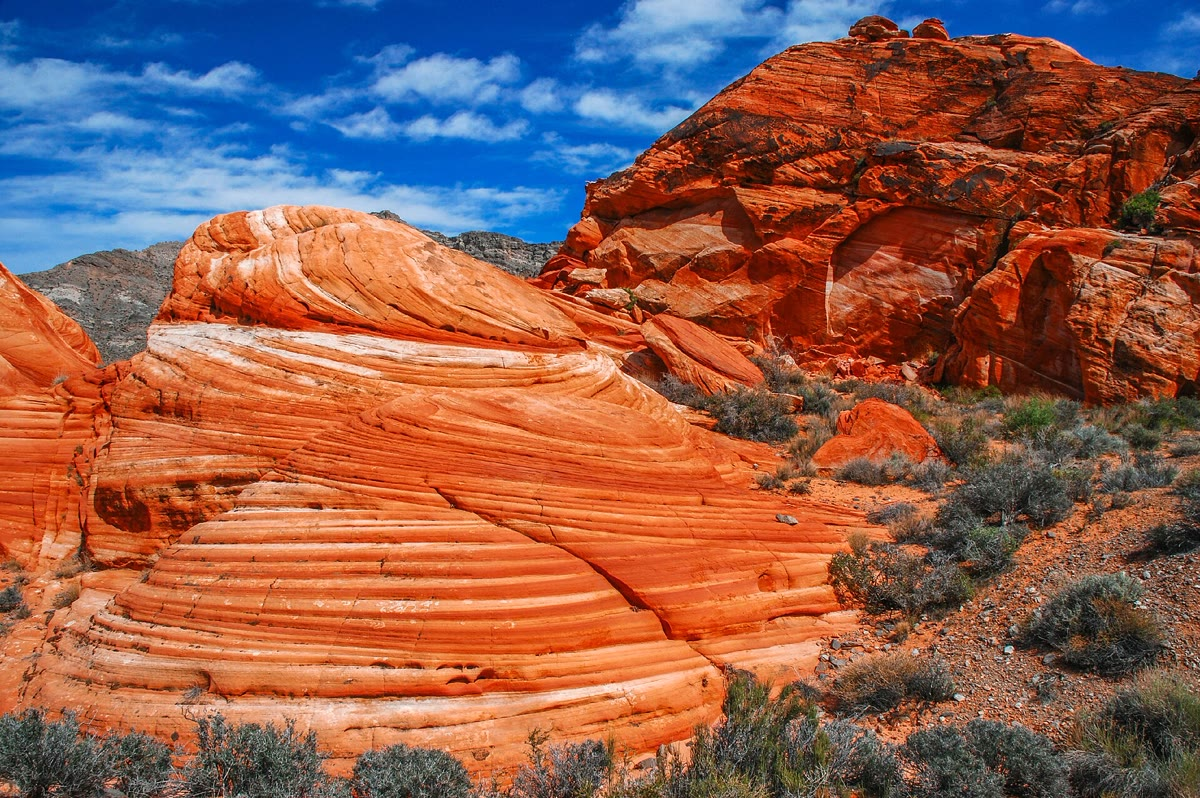
\includegraphics[height=3.6cm]{images/book3/b1-cross-bedding-aztec.jpg}};
\end{tikzpicture}

{\small 左图：攀爬型沙波的几何示意（示意图，角度有所夸大）。
沙波的槽沿以攀爬角 $\theta$ 为\omterm{def:b1:geological-maps:attitude}{倾角}的直线路径移动
（粗线）；相邻两条路径之间保存着前积层的下部，
构成厚度为 $T = L\sin\theta$ 的层组。右图为内华达州
穆迪山的 Aztec 砂岩中的\omterm{def:b1:clastic-sediments:cross-bedding}{交错层理}：倾斜的纹层组，每组顶部
被下一组底部的侵蚀面截断。照片：Chip
Carroon，美国土地管理局，CC~BY-SA~2.0，经维基共享资源提供。}
\label{fig:b1:clastic-sediments:climb}
\end{omfigure}
% ledger: southard:climb, commons:aztec-crossbed

\emph{\omterm{def:b1:clastic-sediments:cross-bedding}{古水流}。}在\omterm{def:b1:geological-maps:geological-map}{露头}上测得的交错层\omterm{def:b1:geological-maps:attitude}{倾向}围绕
水流的平均方向散布，原因是\omterm{def:b1:clastic-sediments:bedform}{沙丘}与\omterm{def:b1:clastic-sediments:bedform}{波痕}的背风面呈弯曲状，
且水流本身也在摆动。其平均值取为矢量平均而非算术平均，
理由见
\cref{prop:b1:field-lab-methods-1:vector-mean}：\omterm{def:b1:spherical-astronomy:horizontal}{方位角}是圆周上的角，
350 与 010 的平均值为 000，而不是 180。

\begin{proposition}[方位角的平均]\label{prop:b1:clastic-sediments:azimuths}
设 $\alpha_1, \ldots, \alpha_N$ 为\omterm{def:b1:spherical-astronomy:horizontal}{方位角}，自北向顺时针量取。
其矢量平均 $\bar\alpha$ 与平均合向量长度 $\bar R$
由下式给出
\[
  S = \sum_{i=1}^N \sin\alpha_i, \quad C = \sum_{i=1}^N \cos\alpha_i, \quad
  \bar\alpha = \operatorname{atan2}(S, C), \quad \bar R = \frac{\sqrt{S^2 + C^2}}{N},
\]
其中 $\operatorname{atan2}(S, C)$ 为正弦与余弦分别与 $S$、$C$ 成比例的角，
取值在 \ang{0} 与 \ang{360} 之间。$\bar R$ 介于
0 与 1 之间，且仅当所有\omterm{def:b1:spherical-astronomy:horizontal}{方位角}都相等时才等于 1。
\end{proposition}

\begin{proof}
\omterm{def:b1:spherical-astronomy:horizontal}{方位角}为 $\alpha$ 的单位矢量，以东为第一分量、北为第二分量，
即 $(\sin\alpha, \cos\alpha)$。$N$ 个单位矢量之和为
$(S, C)$，其方向即矢量平均
（\cref{def:b1:field-lab-methods-1:mean-orientation}），其\omterm{def:b1:spherical-astronomy:horizontal}{方位角}的正弦与余弦分别为
$S/\sqrt{S^2+C^2}$ 与 $C/\sqrt{S^2+C^2}$。由三角不等式，
$N$ 个单位矢量之和的长度至多为 $N$，当且仅当
它们指向同一方向时取等号。
\end{proof}

\begin{method}[由交错层理求古水流]\label{met:b1:clastic-sediments:palaeocurrent}
\begin{enumerate}
  \item 在每一层组上，测量前积层的\omterm{def:b1:geological-maps:attitude}{倾向}，
        选取能显示其真实\omterm{def:b1:geological-maps:attitude}{倾角}的面（或测量\omterm{def:b1:geological-maps:attitude}{走向}与\omterm{def:b1:geological-maps:attitude}{倾角}）。
  \item 测量主层理的\omterm{def:b1:geological-maps:attitude}{产状}；若其倾斜超过数度，
        则绕层理的\omterm{def:b1:geological-maps:attitude}{走向}将每条前积层旋转回水平，
        （旋转可用本科三年级分册中的赤平投影完成）。
  \item 计算经校正\omterm{def:b1:geological-maps:attitude}{倾向}的矢量平均 $\bar\alpha$ 与 $\bar R$，
        （\cref{prop:b1:clastic-sediments:azimuths}）。
  \item 将读数绘成玫瑰图，即\omterm{def:b1:spherical-astronomy:horizontal}{方位角}的圆形直方图，
        以判断它们构成一组还是两组：潮汐水流往复流动，
        会形成\omterm{def:b1:geological-maps:attitude}{倾向}相反的层组，即人字形\omterm{def:b1:clastic-sediments:cross-bedding}{交错层理}，
        此时单一平均值便毫无意义。
\end{enumerate}
\end{method}
% ledger: og:sorting-environments

\emph{其他构造。}若干其他构造记录了沉积条件
以及层的顶底方向。\omterm{def:b1:clastic-sediments:turbidite}{递变层}自下而上变细，底部粗、顶部细，
颗粒随减弱的水流沉降，最粗者先沉降
（\cref{def:b1:clastic-sediments:turbidite}）。泥裂是由上覆层充填的收缩裂缝多边形，
形成于泥在空气中干燥之处，如潮坪与河漫滩上。水流切入下方泥层形成的冲刷痕，
由上方的砂充填，
以内模形式保存于砂岩层的底面，
其形状指示水流的去向。
% ledger: og:sorting-environments

\section{相、河流与三角洲}\label{sec:b1:clastic-sediments:rivers-deltas}

粒度、\omterm{def:b1:clastic-sediments:sorting}{分选}、构造、化石与成分共同构成了沉积岩的
性质，地质学家为此使用一个术语，
即\omterm{def:b1:clastic-sediments:facies}{沉积相}。

\begin{definition}[沉积相，沉积环境]\label{def:b1:clastic-sediments:facies}
称一套沉积岩为\emph{沉积相}\index{沉积相}，
其岩性、粒度、沉积构造与化石使之区别于其他岩体，
这些特征均反映其形成时的条件。
\emph{沉积环境}\index{沉积环境}是沉积物沉积时所处的场所，
包括其物理、化学与生物条件，
例如河道、河漫滩、海滩、三角洲斜坡、
深海海底。
\end{definition}
% ledger: og:sorting-environments

相是一种描述，环境则是一种解释，
且同一种相可以由若干种环境形成：波纹状砂既可沉积于河流中，
也可沉积于潮坪与深海海底。因此，解释依赖于相的组合
以及相的堆叠顺序，这种堆叠顺序随环境在空间中的迁移而变化：
这种堆叠的一般规律以及各类环境的标准模式，
是本科三年级分册的内容。
本章介绍主要的碎屑环境，
以及用以识别它们的垂向序列。

\emph{辫状河与曲流河。}河流大致分为两种主要类型。辫状河
在多条河道中流动，这些河道在砾坝与砂坝周围分叉又汇合；
辫状河在靠近源头处搬运粗粒载荷，例如在山脚下
或冰川前缘，其沉积物为砾石层与粗粒的
交错层砂层，几乎不含泥。曲流河则在单一的
蜿蜒河道中流动。最快的水流沿每个弯道的外侧运动，在那里
侵蚀凹岸；在内侧，水流最慢，沙沉积于
点坝之上。因此曲流侧向迁移，一侧侵蚀，
另一侧堆积；河岸之外的河漫滩只接收
洪水带来的泥。
% ledger: og:rivers

点坝的层序由\omterm{def:b1:clastic-sediments:bedform}{床形}决定。在坝脚
即最深、最快的水流处，水流留下最粗的颗粒，
并形成\omterm{def:b1:clastic-sediments:bedform}{沙丘}；沿缓坡向上，水变浅、流变慢，
沙变细，\omterm{def:b1:clastic-sediments:bedform}{沙丘}让位于\omterm{def:b1:clastic-sediments:bedform}{波痕}
（\cref{sec:b1:clastic-sediments:bedforms}）；在坝顶，点坝过渡为
河漫滩。随着弯道迁移，这些带依次移到下方一带
之上，因此穿过沉积物的钻孔会遇到它们的叠置：
自侵蚀面向上变细直至泥，每次河道经过
便形成一个这样的层序，其厚度约等于造成它的河道的深度。

\emph{三角洲。}当河流进入静止水体时，其水流
扩散并减慢，所携带的负载被卸下：近河口处为粗负载，
远处为细负载。只要河流供给的沉积物多于波浪和潮汐能搬走的量，三角洲便向前生长，即进积。
波浪和潮汐对供给的作用，
决定了三角洲的形状。

\begin{definition}[河控、浪控和潮控三角洲]\label{def:b1:clastic-sediments:delta}
当河流的供给压倒波浪和潮汐时，三角洲为\emph{河控}\index{河控三角洲}，
其分流河道受自身天然堤约束，
向海中伸出长长的砂指；三角洲为
\emph{浪控}\index{浪控三角洲}，当波浪将
送达河口的砂改造为沿光滑弧形的
海岸分布的海滩和滩脊时；三角洲为
\emph{潮控}\index{潮控三角洲}，当进出河口的潮流
将其砂塑造为与流向平行的砂坝和脊，彼此被漏斗形河道隔开。
\end{definition}
% ledger: og:deltas

\begin{omfigure}
\begin{tikzpicture}[font=\footnotesize, >={Stealth[length=4pt]}]
% meander in plan view (schematic) and the fining-upward log of a point bar
\begin{scope}[yscale=0.8]
  \fill[green!8] (-0.2,-0.4) rectangle (7.2,4.4);
  \draw[omSea!80!black, line width=9pt] plot[smooth, tension=0.7] coordinates {(0,3.6) (1.4,3.7) (2.6,2.8) (2.3,1.4) (3.2,0.5) (4.6,0.8) (5.0,2.2) (5.6,3.4) (7.0,3.5)};
  \draw[omSea!45, line width=7pt] plot[smooth, tension=0.7] coordinates {(0,3.6) (1.4,3.7) (2.6,2.8) (2.3,1.4) (3.2,0.5) (4.6,0.8) (5.0,2.2) (5.6,3.4) (7.0,3.5)};
  % point bars (inside of bends) with scroll lines
  \foreach \r in {0.25,0.45,0.65} {\draw[brown!60!black, densely dotted] (3.45,1.15) ++(200:\r) arc[start angle=200, end angle=340, radius=\r];}
  \fill[brown!25, opacity=0.8] (3.45,1.25) ellipse[x radius=0.55, y radius=0.35];
  \node[align=center] at (3.45,1.95) {点坝 \\ （沉积）};
  \fill[brown!25, opacity=0.8] (1.75,2.75) ellipse[x radius=0.4, y radius=0.45];
  \node[align=center] at (1.3,1.95) {点坝};
  \draw[red!60!black, thick] (2.9,0.2) .. controls (3.3,0.0) and (4.3,0.15) .. (4.85,0.6);
  \node[red!60!black, anchor=north] at (4.0,0.0) {凹岸侵蚀};
  \draw[->, black!70] (5.9,3.0) -- (6.7,3.15) node[right] {水流};
  \node[anchor=north west, black!60] at (5.2,1.3) {河漫滩};
  \node[font=\footnotesize] at (3.5,-0.85) {(a) 曲流，平面图};
\end{scope}
\begin{scope}[xshift=9.2cm, yshift=-0.3cm, yscale=0.8]
  % log: x width = grain size; y = height
  \draw[lith shale] (0,3.6) rectangle (0.8,4.6);
  \draw[lith sandstone] (0,2.6) rectangle (1.2,3.6);
  \draw[lith sandstone] (0,0.6) rectangle (1.7,2.6);
  \draw[lith conglomerate] (0,0) rectangle (2.2,0.6);
  \draw[very thick, red!60!black] (0,0) -- (2.2,0);
  % cross-bed symbols
  \foreach \y in {0.9,1.5,2.1} {\draw[black!70] (0.3,\y) .. controls (0.6,\y+0.05) and (0.9,\y+0.25) .. (1.2,\y+0.4);}
  \foreach \x in {0.2,0.5,0.8} {\draw[black!70] (\x,3.0) -- ++(0.12,0.1) -- ++(0.12,-0.1);}
  \node[anchor=west, align=left] at (2.4,4.1) {河漫滩泥、\\ 根系、泥裂};
  \node[anchor=west, align=left] at (2.4,3.1) {细砂、波痕 \\ 交错层理};
  \node[anchor=west, align=left] at (2.4,1.6) {中至粗砂、\\ 沙丘交错层理};
  \node[anchor=west, align=left] at (2.4,0.3) {侵蚀面上的 \\ 砾石滞留};
  \draw[->] (-0.35,0) -- (-0.35,4.6) node[above] {向上};
  \draw[<->, black!60] (-0.7,0) -- node[above, rotate=90, font=\scriptsize] {河道深度} (-0.7,3.6);
  \node[font=\footnotesize] at (1.8,-0.5) {(b) 点坝层序};
\end{scope}
\end{tikzpicture}

{\small (a)~曲流河（示意）：水流侵蚀每个弯道的凹岸，
并在其内侧的点坝上沉积砂；弧形的迁移线表示
点坝的相继位置。(b)~迁移中的点坝留下的层序，
每层的宽度与其粒度成正比（示意）。它
向上变细，其厚度记录了河道的深度。}
\label{fig:b1:clastic-sediments:point-bar}
\end{omfigure}
% ledger: og:rivers, southard:phase-diagram

三个\omterm{def:b1:rock-forming-minerals:solid-solution}{端元}是三角形的三个顶点，任一三角洲都可按
三种过程的相对强弱置于其中。
密西西比河的鸟足状三角洲，其长长的砂指伸入墨西哥湾，
（\cref{ch:b1:erosion-transport}）是典型的\omterm{def:b1:clastic-sediments:delta}{河控三角洲}；
尼罗河的三角洲有光滑弧形的海滩，属\omterm{def:b1:clastic-sediments:delta}{浪控三角洲}；
恒河与布拉马普特拉河的三角洲是世界上最大的三角洲，属\omterm{def:b1:clastic-sediments:delta}{潮控三角洲}。
% ledger: og:deltas

\begin{omfigure}
\begin{tikzpicture}[font=\footnotesize]
% delta classification triangle (schematic) and the Lena delta from Landsat
\begin{scope}[yscale=0.82]
  \coordinate (R) at (2.6,4.5); \coordinate (W) at (0,0); \coordinate (T) at (5.2,0);
  \fill[omDef!8] (R) -- (W) -- (T) -- cycle;
  \draw[thick] (R) -- (W) -- (T) -- cycle;
  \node[above, align=center] at (R) {\textbf{河控}\\ 长条状砂指、天然堤};
  \node[below, align=center] at (W) {\textbf{浪控}\\ 光滑的海滩脊};
  \node[below, align=center] at (T) {\textbf{潮控}\\ 沿流向的砂坝};
  \fill[omThm] (2.6,2.9) circle[radius=2pt] node[below=1pt] {密西西比河};
  \fill[omThm] (0.75,0.4) circle[radius=2pt] node[above right=0pt] {尼罗河};
  \fill[omThm] (4.4,0.4) circle[radius=2pt] node[above left=0pt, align=right] {恒河--\\ 布拉马普特拉河};
\end{scope}
\node[anchor=south west, inner sep=0] at (7.2,-0.9) {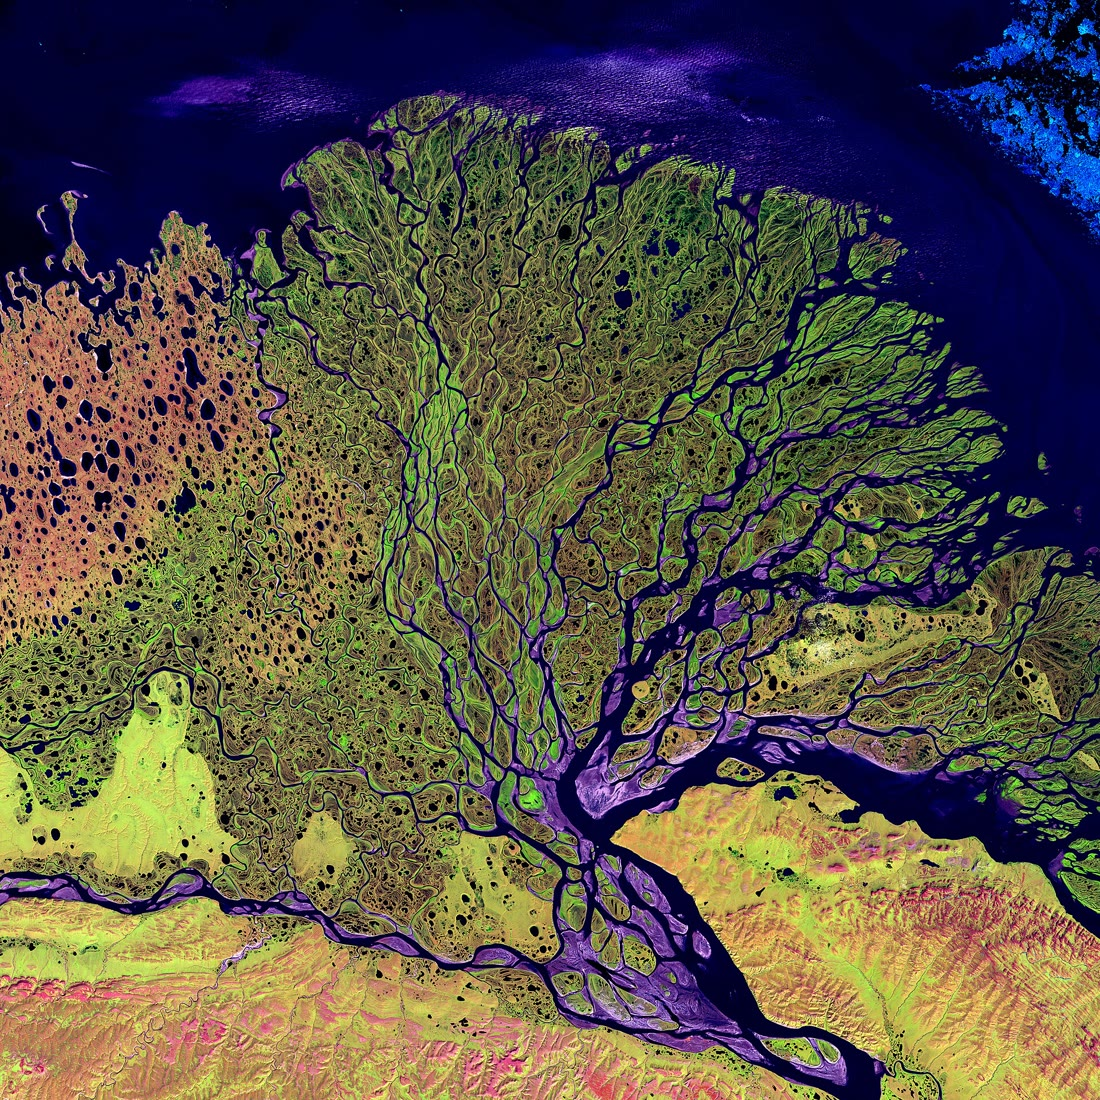
\includegraphics[height=5.2cm]{images/book3/b1-lena-delta.jpg}};
\end{tikzpicture}

{\small 左：三角洲的三个\omterm{def:b1:rock-forming-minerals:solid-solution}{端元}，按塑造它们的过程划分
（示意；三个实例的位置仅供参考）。右：西伯利亚的勒拿河三角洲，
伸入拉普捷夫海（上方）；河流自右下方进入，
分为数百条分流河道。Landsat~7
假彩色图像，拍摄于 2000 年 2 月 27 日，美国地质调查局，公有领域，
经维基共享资源获取。}
\label{fig:b1:clastic-sediments:deltas}
\end{omfigure}
% ledger: og:deltas, commons:lena-delta

\emph{向上变粗的层序。}在河口前方，三角洲具有
平缓倾斜的前缘，即三角洲前缘，其向海一侧过渡为
前三角洲，那里只有泥从悬浮中沉降下来。随着三角洲进积，各带
都向其前方的一带推进：在三角洲平原上的钻孔，
自下而上依次遇到前三角洲的纹层状泥、
下三角洲前缘的粉砂与砂互层，河口坝的\omterm{def:b1:clastic-sediments:cross-bedding}{交错层理}砂，
顶部则被三角洲平原的河道切割。
该层序向上变粗，与点坝的层序正好相反，其厚度约等于
三角洲堆积时所在水体的深度。其速率与
三角洲前缘的几何形态有关。

\begin{proposition}[进积与堆积]\label{prop:b1:clastic-sediments:progradation}
设坡度为常数 $\alpha$ 的三角洲前缘，在海平面不变的条件下以
速度 $v$ 水平推进且形状不变。前缘下方的一个固定点
则以竖直速率接收沉积物，
\[
  a = v\,\tan\alpha,
\]
而厚度为 $h$ 的三角洲前缘层序在该点
堆积所需的时间为 $h/(v\tan\alpha)$。
\end{proposition}

\begin{proof}
在时间 $\mathrm dt$ 内，前缘向前推进 $v\,\mathrm dt$。在
倾斜表面下方的一个固定点处，表面抬升的高度等于
相距水平距离 $v\,\mathrm dt$ 的前缘两点之间的高差，
即 $v\,\mathrm dt\,\tan\alpha$，由此得出速率。前缘经过
该点、表面抬升 $h$ 所需时间为 $h/a$。
\end{proof}

三角洲前缘坡度平缓，故 $\tan\alpha$ 很小：三角洲前缘的
推进速度远快于其下任一点沉积物的堆积速度
（见\cref{exo:b1:clastic-sediments:12}）。

\begin{inthelab}[描述岩芯]
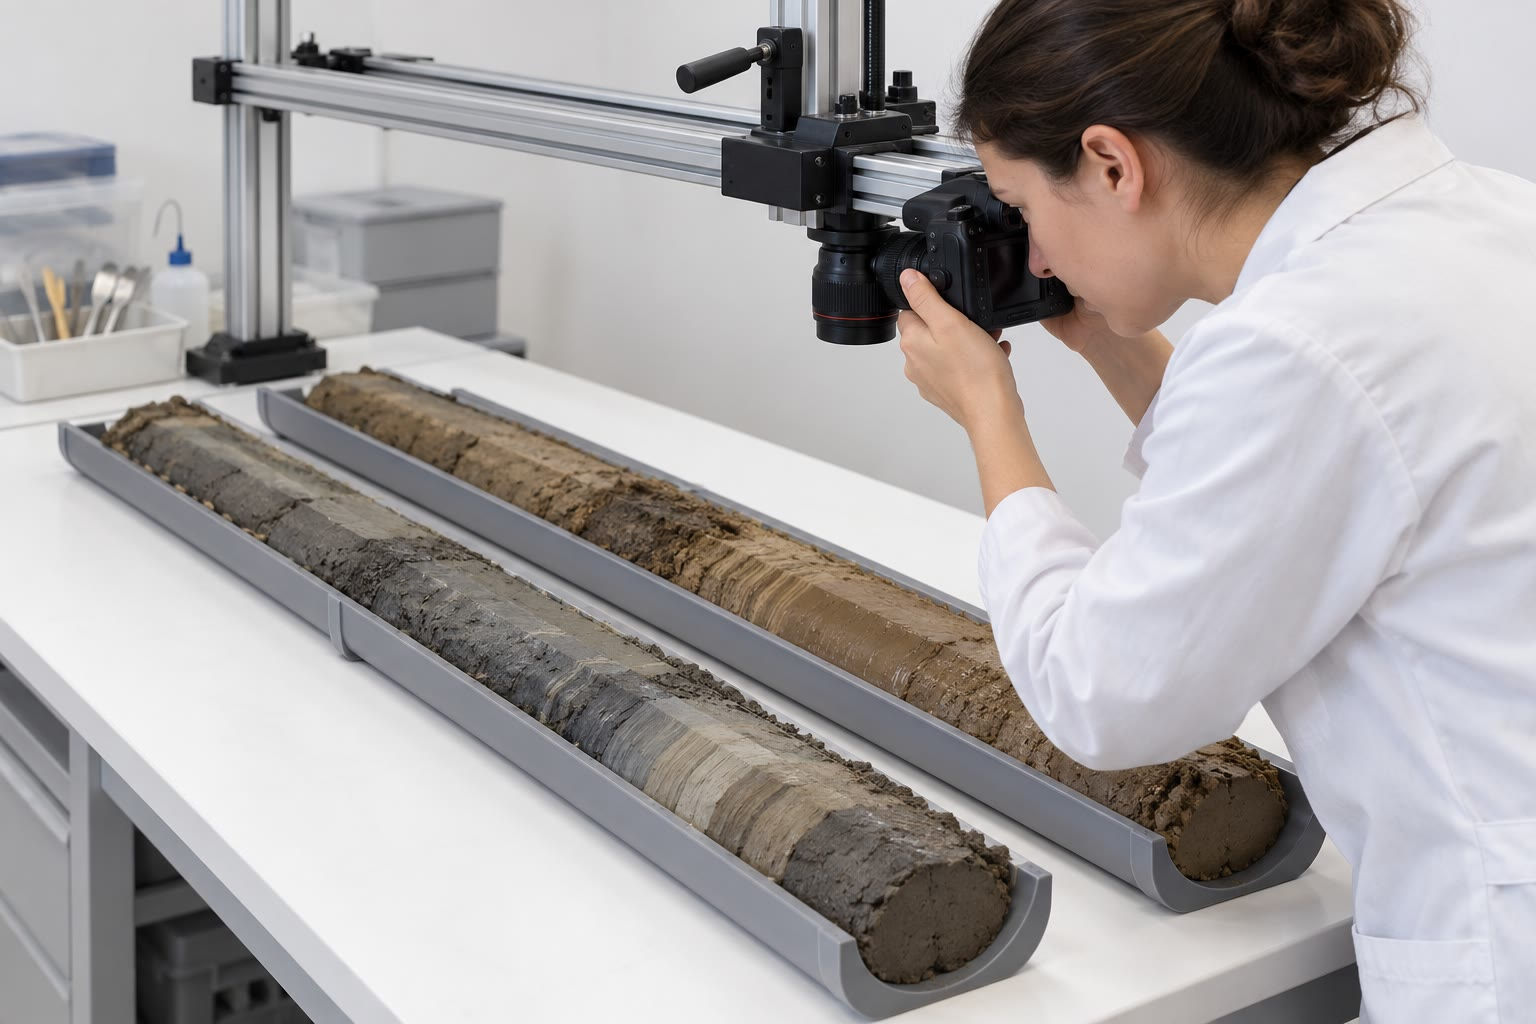
\includegraphics[width=0.3\linewidth]{images/book3/ai/b1-core-lab.jpg}\hfill
\begin{minipage}[b]{0.67\linewidth}
钻探取出的沉积物或岩石圆柱体按深度顺序
摆放在托盘中，纵向剖开，并在均匀光照下拍照，趁其
尚未干燥变色。沉积学家随后绘制岩芯柱状图，
逐米记录岩性、各层粒度（柱状图的宽度）、
构造（\omterm{def:b1:clastic-sediments:cross-bedding}{交错层理}、纹层、递变、虫孔）、
\omterm{def:b1:geological-maps:geological-map}{地质界线}（突变或渐变）、颜色与化石。取样用于
粒度分析和\omterm{def:b1:field-lab-methods-1:thin-section}{薄片}。岩芯只是一个狭窄的观察窗：
除非岩芯经过定向，否则交错层的方向无从得知，
岩层的横向延伸范围须依靠其他钻孔来确定。
\end{minipage}

\smallskip
{\small 在沉积学实验室中摆放、待拍照的岩芯（
AI 插图）。}
\end{inthelab}

\section{海岸与陆架}\label{sec:b1:clastic-sediments:shoreline}

沿三角洲之间的海岸，河流带来的砂受到波浪与潮汐的
塑造。海滩是经冲流再改造的砂，冲流是
每个波浪破碎后沿海滩上下流动的薄层水流：颗粒被反复
搬运，细粒被带向近岸之外，海滩砂属于
所有沉积物中\omterm{def:b1:clastic-sediments:sorting}{分选}和磨圆最好的一类。其纹层由冲流
沉积形成，向海微倾。在许多低平海岸，砂形成障壁岛，
即由海滩与风成\omterm{def:b1:clastic-sediments:bedform}{沙丘}组成的长条形脊，与大陆之间
隔着泻湖。泻湖水体平静，沉积细粒，通过潮汐
通道与大海相连。

在潮汐强而波浪弱的地方，海岸边缘镶嵌着潮坪，
潮坪每日被淹没与出露两次。其沉积由低潮线附近的砂
（水流最强处）过渡到高潮线附近的泥（
缓流使黏土沉降）；其沉积中，往复水流由
人字形\omterm{def:b1:clastic-sediments:cross-bedding}{交错层理}显示，干燥由泥裂记录，水流与缓流的交替
则表现为覆于波纹砂之上的薄层泥。

在近海，陆架仅受波浪扰动至随波浪尺度增大而加深的水深，
以上的砂被筛选搬运，以下则是泥沉降，
但风暴期间，较大波浪可达更深处，沉积形成
具平缓起伏纹层的砂层，称为丘状\omterm{def:b1:clastic-sediments:cross-bedding}{交错层理}。
因此陆架层序常为晴天泥与风暴砂互层，
且越近岸越厚、越粗。
% ledger: og:sorting-environments, folk:maturity

\section{深海碎屑沉积}\label{sec:b1:clastic-sediments:deep-sea}

砂与砾石也抵达深海海底，深度达数千米，
离陆地数百千米。它们由
从未有人完整观测过的水流搬运至此：这些致密、
携带大量沉积物的水流，在清澈的海水之下沿大陆坡向下流动。

\begin{history}[海底电缆，1929 年]
1929 年 11 月 18 日，一次\omterm{def:b1:earthquake-source:mw}{矩震级}为 7.2 的地震袭击了
纽芬兰以南、大浅滩南缘的大陆坡。一次滑塌
约 \qty{200}{km^3} 的沉积物在斜坡上滑动，海啸
在纽芬兰海岸造成 28 人遇难。横跨海底铺设的十二条
电报电缆断裂，其中数条多处断裂。靠近震中的电缆
立即断裂；其余电缆位于更南、更深之处，
在随后数小时内依次断裂，顺序沿斜坡由近及远。1952 年，布鲁斯·希真与莫里斯·尤因
研究了断裂的时间，给出解释：滑塌已转化为
一股\omterm{def:b1:clastic-sediments:turbidite}{浊流}，沿斜坡向下穿过深海平原，
流程超过 480 英里，每经过一条电缆便将其切断。由断裂时间与
距离，他们估算其在上部大陆隆的速度约为 50 节，
该处坡度约为 \qty{0.5}{\percent}，而在
最后一条电缆处（距其起源约 400 英里）仍为 12 节。他们认为，
随着速度减慢，它必然在平原上沉积出自下而上逐渐变细的\omterm{def:b1:clastic-sediments:turbidite}{递变层}。
\end{history}
% ledger: nrcan:grand-banks, he52:grand-banks

五十节合 \qty{25.7}{m.s^{-1}}，超过 \qty{90}{km.h^{-1}}，
相当于普通公路上一辆汽车的车速；12 节合 \qty{6.2}{m.s^{-1}}；480 英里约合
\qty{770}{km}。断裂的时间还首次给出了这种流动的实测速度，
此前这种流动只能根据其沉积物和水槽实验推断。
% ledger: he52:grand-banks

\begin{definition}[浊流、浊积岩、递变层]\label{def:b1:clastic-sediments:turbidite}
称\emph{浊流}\index{浊流}为一股水流，它因所悬浮的沉积物而
密度大于周围的水，
沿斜坡在该水体之下流动，颗粒
依靠自身运动产生的湍流而保持悬浮。称\emph{浊积岩}\index{浊积岩}为
浊流的沉积物。称\emph{递变层}\index{递变层}为
粒度自底至顶逐渐减小的层。
\end{definition}
% ledger: og:sorting-environments, he52:grand-banks

\omterm{def:b1:clastic-sediments:turbidite}{浊流}靠自身运动维持：其悬浮物使它较重而流动，
又因流动而保持悬浮。在陡坡上，它能从床面带走更多
沉积物，密度增大并加速；在深海平原的缓坡上，
它减速、卸下所携带的沉积物，随之消亡。

\begin{proposition}[浊流的速度]\label{prop:b1:clastic-sediments:turbidity}
设厚度为 $h$、密度为 $\rho + \Delta\rho$ 的\omterm{def:b1:clastic-sediments:turbidite}{浊流}，
沿坡度为 $S$ 的斜坡在密度为 $\rho$ 的水下稳定流动。若床面及其上方水体对其
的阻力为单位面积上的 $\tau = \rho\,C_f\,U^2$，其中 $C_f$
为无量纲的摩擦系数，则其平均速度为
\[
  U = \sqrt{\frac{\Delta\rho}{\rho}\,\frac{g\,h\,S}{C_f}} .
\]
\end{proposition}

\begin{proof}
证明采用深度–坡度乘积的论证，
（见\cref{prop:b1:erosion-transport:depth-slope}），以超重代替重量。
即超出部分的重力。单位面积的\omterm{def:b1:clastic-sediments:turbidite}{浊流}柱重 $(\rho +
\Delta\rho) g h$，其排开的水重 $\rho g h$：在周围的水中，
只有超出部分 $\Delta\rho\,g\,h$ 将其拉向坡下，沿坡的
分量为 $\Delta\rho\,g\,h\,S$。稳定流动时，此力与
阻力 $\rho C_f U^2$ 平衡，因此 $U^2 = (\Delta\rho/\rho)\,g\,h\,S/C_f$。
\end{proof}

阻力定律 $\tau = \rho C_f U^2$ 对速度是二次的，与
水力学中湍流的阻力定律相同（见物理学教材），而 $C_f$ 由
实验确定。该公式忽略了\omterm{def:b1:clastic-sediments:turbidite}{浊流}混入自身上表面的水，
这些水会使其稀释并减速。公式表明了三个因素的作用：
厚度加倍、密度加倍，或坡度加倍（即更陡），
\omterm{def:b1:clastic-sediments:turbidite}{浊流}的速度变为原来的 $\sqrt 2$ 倍。若悬浮体中
石英颗粒占其体积的比例为 $c$，则 $\Delta\rho/\rho = 1.65\,c$
（见\cref{sec:b1:erosion-transport:settling}），除非流动很浓，否则该值很小；
这正是\omterm{def:b1:clastic-sediments:turbidite}{浊流}与河流的不同之处：河流中是水的全部重量
而非微小的超重驱动流动。要在坡度为 0.5\% 的斜坡上达到
1929 年的 50 节，\omterm{def:b1:clastic-sediments:turbidite}{浊流}需要很大的厚度与密度超重的乘积
（见\cref{exo:b1:clastic-sediments:11}）。

\emph{鲍马层序。} 1962 年，阿诺德·鲍马描述了古代深海层序
中砂岩层的内部序列，将其分为五段，自下而上依次标记为
A：块状或递变砂，常位于侵蚀底面之上；B：砂，
具平行层理；C：具\omterm{def:b1:clastic-sediments:bedform}{波痕}\omterm{def:b1:clastic-sediments:cross-bedding}{交错层理}的细砂，常见卷曲层理；
D：具纹层的粉砂，向泥递变；E：泥。该序列被解释为
单一衰减水流经过某一点时留下的记录：水流减速时，
先整体沉积最粗的颗粒，然后形成上部的平床层，
接着是\omterm{def:b1:clastic-sediments:bedform}{波痕}，最后让粉砂和黏土沉降。完整的层序很少见：
上部各段常被下一股水流侵蚀，而远离物源、水流较弱的地方，
下部各段则缺失。
% ledger: og:sorting-environments, shanmugam:bouma

\begin{omfigure}
\begin{tikzpicture}[font=\footnotesize]
% Bouma sequence: log (schematic) and a labelled photograph
\begin{scope}
  \draw[lith shale] (0,4.0) rectangle (0.7,4.8);
  \draw[lith shale] (0,3.3) rectangle (0.9,4.0);
  \draw[lith sandstone] (0,2.2) rectangle (1.3,3.3);
  \draw[lith sandstone] (0,1.2) rectangle (1.6,2.2);
  \draw[lith sandstone] (0,0) rectangle (2.0,1.2);
  \draw[very thick, red!60!black] (0,0) .. controls (0.6,-0.12) and (1.4,0.1) .. (2.0,0);
  \foreach \y in {1.4,1.6,1.8,2.0} {\draw[black!70] (0.1,\y) -- (1.5,\y);}
  \foreach \x in {0.15,0.5,0.85} {\draw[black!70] (\x,2.55) .. controls (\x+0.12,2.75) .. (\x+0.3,2.6);}
  \foreach \y in {3.45,3.6,3.75,3.9} {\draw[black!60] (0.1,\y) -- (0.8,\y);}
  \foreach \x/\y in {0.4/0.3, 0.9/0.5, 1.4/0.25, 0.6/0.8, 1.2/0.9} {\fill[black!60] (\x,\y) circle[radius=0.06];}
  \node[anchor=west] at (2.2,4.4) {E \quad 泥};
  \node[anchor=west] at (2.2,3.65) {D \quad 纹层粉砂至泥};
  \node[anchor=west] at (2.2,2.75) {C \quad 波痕交错层理};
  \node[anchor=west] at (2.2,1.7) {B \quad 平行层理};
  \node[anchor=west] at (2.2,0.6) {A \quad 递变砂};
  \node[anchor=west, red!60!black] at (2.2,-0.15) {侵蚀底面，底面痕};
  \draw[->] (-0.3,0) -- (-0.3,4.8) node[above] {上};
\end{scope}
\node[anchor=south west, inner sep=0] at (6.9,-0.3) {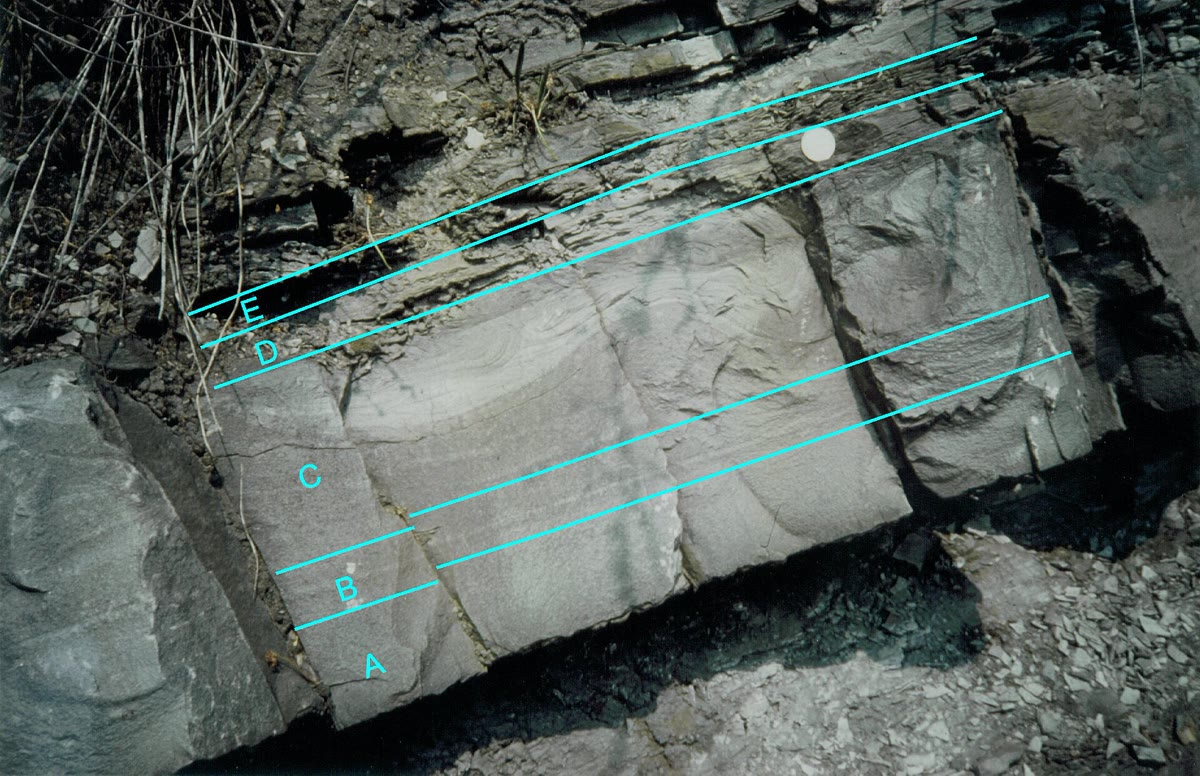
\includegraphics[height=5.2cm]{images/book3/b1-turbidite-bouma.jpg}};
\end{tikzpicture}

{\small 左：鲍马层序的五个段，每段的宽度
与其粒度成比例（示意）。右：德国 Becke-Oese 的上泥盆统\omterm{def:b1:clastic-sediments:turbidite}{浊积岩}层，
摄影者标出了 A 至 E 各段；
硬币给出比例尺。照片：Jo Weber，CC~BY-SA~3.0，经
维基共享资源提供。}
\label{fig:b1:clastic-sediments:bouma}
\end{omfigure}
% ledger: og:sorting-environments, shanmugam:bouma, commons:bouma-becke-oese

鲍马层序成为\omterm{def:b1:clastic-sediments:turbidite}{浊积岩}的标准模型，成千上万的古代深海砂岩都依据它
来解释。但这一解释存在争议：沿坡流动的水流、深层潮流和内
波同样能形成具\omterm{def:b1:clastic-sediments:bedform}{波痕}和纹层的砂，一些沉积学家认为，
许多被当作\omterm{def:b1:clastic-sediments:turbidite}{浊积岩}的层（包括标准产地的部分层）
实为其他水流沉积而成。
现代海洋中观察到的\omterm{def:b1:clastic-sediments:turbidite}{浊流}很少，
而古代\omterm{def:b1:clastic-sediments:turbidite}{浊积岩}则以千计。
% ledger: shanmugam:bouma

并非所有深海碎屑岩都是\omterm{def:b1:clastic-sediments:turbidite}{浊积岩}。等深流是缓慢的深层水流，
沿大陆坡的等深线流动，把坡上的沉积物
重新搬运，形成光滑、细长的沉积体，即等深流积岩。而远离
大陆、\omterm{def:b1:clastic-sediments:turbidite}{浊流}与等深流都无法到达的地方，海底
只接收从上方水体沉降下来的物质：浮游生物的壳体
和最细的风吹尘埃，即
下一章所讨论的远洋沉积（见\cref{ch:b1:chemical-biogenic-sediments}）。
% ledger: og:sorting-environments

\section{练习}

\begin{exercise}[$\star$]\label{exo:b1:clastic-sediments:1}
将下列直径换算为 phi 单位：\qty{0.18}{mm}、
\qty{0.75}{mm}、\qty{3}{mm}、\qty{0.012}{mm} 和 \qty{150}{mm}，保留两位小数，并说明
每个直径所属的类别（见\cref{tab:b1:clastic-sediments:classes}）。
% ledger: folk:wentworth-classes
\end{exercise}

\begin{exercise}[$\star$]\label{exo:b1:clastic-sediments:2}
某河砂的累积曲线给出 $\varphi_5 = 0.62$、$\varphi_{16} =
1.05$、$\varphi_{50} = 1.71$、$\varphi_{84} = 2.43$ 和 $\varphi_{95} = 2.98$。
求其图解平均值（分别以 phi 单位和毫米表示），以及其包容
图解标准差，并说明其粒级和\omterm{def:b1:clastic-sediments:sorting}{分选}程度。
% ledger: folk:graphic-measures, folk:sorting-classes
\end{exercise}

\begin{exercise}[$\star$]\label{exo:b1:clastic-sediments:3}
\omterm{def:b1:clastic-sediments:bedform}{波痕}高 \qty{2}{cm}，以每分钟 \qty{1}{cm} 的速度在石英砂层上迁移，
砂层孔隙度为 \num{0.4}。利用\cref{prop:b1:clastic-sediments:migration}，
求单位宽度上\omterm{def:b1:erosion-transport:load}{推移质}的体积（以 \si{m^2.s^{-1}} 为单位），以及
一天内沿一米长的波峰输运的石英质量（石英密度 $\qty{2650}{kg.m^{-3}}$）。
% ledger: hom:quartz
\end{exercise}

\begin{exercise}[$\star$]\label{exo:b1:clastic-sediments:4}
一节即每小时一海里（\qty{1852}{m}）。(a)~
将\omterm{def:b1:clastic-sediments:turbidite}{浊流}估计的 50 节和 12 节速度换算为米每秒（该\omterm{def:b1:clastic-sediments:turbidite}{浊流}发生于
1929 年）。(b)~以 12 节速度运动的水流需要多长时间才能通过 \qty{100}{km}？
(c)~将 480 和 400 英里换算为千米（一英里为 \qty{1.609}{km}）。
% ledger: he52:grand-banks
\end{exercise}

\begin{exercise}[$\star\star$]\label{exo:b1:clastic-sediments:5}
(a)~利用
\cref{prop:b1:clastic-sediments:normal}的证明中给出的正态分布百分位数，求图解标准差
$(\varphi_{84} - \varphi_{16})/2$，以及
$(\varphi_{95} - \varphi_5)/3.3$ 的估计值，该正态分布的标准差为
$\sigma$。(b)~为什么两者对实际沉积物可能不一致？哪一类
沉积物使两者差异最大？
\end{exercise}

\begin{exercise}[$\star\star$]\label{exo:b1:clastic-sediments:6}
一套爬升\omterm{def:b1:clastic-sediments:bedform}{波痕}沉积，其层组厚 \qty{1.5}{cm}（垂直于界面测量），
由间距为 \qty{15}{cm} 的\omterm{def:b1:clastic-sediments:bedform}{波痕}形成。(a)~求爬升角。(b)~若\omterm{def:b1:clastic-sediments:bedform}{波痕}以
每分钟 \qty{0.5}{cm} 的速度移动，则床面抬升速率为多少（以厘米每
小时表示）？
(c)~这样的速率说明了水流的什么情况？
% ledger: southard:climb
\end{exercise}

\begin{exercise}[$\star\star$]\label{exo:b1:clastic-sediments:7}
六个\omterm{def:b1:clastic-sediments:cross-bedding}{交错层理}的\omterm{def:b1:geological-maps:attitude}{倾向}（已校正层面倾斜），分别为
350、020、005、340、015 和 030。(a)~求其算术平均值。(b)~求
其矢量平均值及 $\bar R$。(c)~解释二者的差异。
\end{exercise}

\begin{exercise}[$\star\star$]\label{exo:b1:clastic-sediments:8}
三块砂岩在\omterm{def:b1:field-lab-methods-1:thin-section}{薄片}中进行了观察。A 含有 \qty{12}{\percent} 的
黏土基质，颗粒为棱角状的石英、\omterm{def:b1:rock-forming-minerals:groups}{长石}和岩屑。B 含有
\qty{2}{\percent} 的黏土，$\sigma_I = 0.40\,\varphi$，石英颗粒的
磨圆度为 \num{2.2}（按福克标度）。C 不含黏土，$\sigma_I =
0.30\,\varphi$，石英颗粒磨圆度为 \num{3.6}，且石英含量
为 \qty{98}{\percent}。求各样品的\omterm{def:b1:clastic-sediments:maturity}{结构成熟度}，并推测各自的
\omterm{def:b1:clastic-sediments:facies}{沉积环境}。
% ledger: folk:maturity
\end{exercise}

\begin{exercise}[$\star\star$]\label{exo:b1:clastic-sediments:9}
(a)~求水深 \qty{0.3}{m} 的水流在
\qty{1.5}{m.s^{-1}} 时的弗劳德数，以及水深 \qty{2}{m} 的河流在 \qty{1.0}{m.s^{-1}} 时的弗劳德数（$g
= \qty{9.81}{m.s^{-2}}$）。(b)~对流速为
\qty{1.5}{m.s^{-1}} 的水流，弗劳德数达到 1 时的水深为多少，以及水深 \qty{2}{m} 的河流
需要多大流速？(c)~为什么反\omterm{def:b1:clastic-sediments:bedform}{沙丘}常见于从海滩上漫流而下的薄水层中，
而在大河中却少见？
% ledger: southard:ripples-dunes
\end{exercise}

\begin{exercise}[$\star\star\star$]\label{exo:b1:clastic-sediments:10}
某砂样的筛分分析结果，以整 phi 粒级划分，从 $-1$ 到
$5\,\varphi$，各粒级的质量百分数依次为 2、8、30、40、15 和 5。(a)~用
矩法求以 phi 为单位的平均值和标准差，并
说明其\omterm{def:b1:clastic-sediments:sorting}{分选}等级。(b)~作累积曲线，读取 $\varphi_5$、$\varphi_{16}$、
$\varphi_{50}$、$\varphi_{84}$ 和 $\varphi_{95}$ 用线性插值法读出，并
求 $M_z$ 和 $\sigma_I$。(c)~比较两种结果。
% ledger: folk:graphic-measures, folk:sorting-classes
\end{exercise}

\begin{exercise}[$\star\star\star$]\label{exo:b1:clastic-sediments:11}
在\cref{prop:b1:clastic-sediments:turbidity}中取 $C_f = 0.003$。(a)~一股
厚 \qty{50}{m} 的\omterm{def:b1:clastic-sediments:turbidite}{浊流}，其密度超量为
\qty{2}{\percent}，沿坡度为 \num{0.005} 的斜坡向下流动：求其速度（以米
每秒和节表示）。(b)~厚度与相对密度超量的乘积应为多大，
才能在同一坡度上得到 1929 年的 50 节速度？(c)~与
(a) 中相同的\omterm{def:b1:clastic-sediments:turbidite}{浊流}到达坡度为 \num{0.001} 的斜坡时，求其新速度，设
其余条件不变。其搬运的沉积物会怎样变化？
% ledger: he52:grand-banks
\end{exercise}

\begin{exercise}[$\star\star\star$]\label{exo:b1:clastic-sediments:12}
某河每年向其三角洲输送 \qty{50}{Mt} 沉积物，其中
\qty{70}{\percent} 沉积于宽 \qty{100}{km} 的三角洲前缘，该前缘
向水深 \qty{30}{m} 的水体中推进。沉积物的体积密度为
\qty{2000}{kg.m^{-3}}。(a)~每年增加的体积为多少？(b)~若该体积
充满前缘全宽上的整个水深，则前缘以多快的速度
推进？(c)~三角洲前缘坡度为 \ang{0.5}，则在其下方某固定点处，
沉积物的堆积速率为多少，并需多少年，
该处才形成向上变粗的层序？
\end{exercise}

\section{问题：读取三角洲岩芯}

\begin{problem}[{周末问题——穿过古三角洲的钻孔，由
粒度推断其河流的流向}]
\label{pb:b1:clastic-sediments:1}
% values: calc/ch21.py; the borehole, its beds, ages and readings are invented
一口钻孔穿过 \qty{24}{m} 厚的砂岩和泥岩，它们由
一个古三角洲沉积形成。地质学家自下而上描述了四个岩层单元，并
分析了每个单元的一个样品。

\smallskip
\begin{center}\small
\begin{tabular}{@{}llccccc@{}}
\hline
单元（自底向上的深度） & 描述 & $\varphi_5$ & $\varphi_{16}$ & $\varphi_{50}$ & $\varphi_{84}$ & $\varphi_{95}$ \\
\hline
1（0--8 米） & 纹层状灰色泥岩 & 4.2 & 5.0 & 6.6 & 8.4 & 9.6 \\
2（8--16 米） & 粉砂岩与砂岩互层 & 1.9 & 2.4 & 3.4 & 4.6 & 5.5 \\
3（16--21 米） & \omterm{def:b1:clastic-sediments:cross-bedding}{交错层理}砂岩 & 0.9 & 1.25 & 1.8 & 2.35 & 2.7 \\
4（21--24 米） & 含砾砂岩，底部为侵蚀面 & $-1.8$ & $-0.8$ & 0.9 & 2.1 & 2.9 \\
\hline
\end{tabular}
\end{center}

\medskip
\noindent\textbf{第一部分——粒度。}
\begin{enumerate}
  \item 计算每个单元的图解\omterm{def:b1:clastic-sediments:sorting}{平均粒径} $M_z$，分别以 phi 单位和
        毫米表示。
  \item 计算每个单元的包容图解标准差
        $\sigma_I$。
  \item 指出每个单元\omterm{def:b1:clastic-sediments:sorting}{平均粒径}所属的粒级及其\omterm{def:b1:clastic-sediments:sorting}{分选}程度。
  \item 哪个单元\omterm{def:b1:clastic-sediments:sorting}{分选}最好？为什么河口坝的
        \omterm{def:b1:clastic-sediments:sorting}{分选}比前三角洲泥更好？
  \item 在 $\varphi_{50}$ 与 $\varphi_{84}$ 之间作线性插值，
        估算单元~1 中黏土级颗粒（小于
        $8\,\varphi$）所占的百分比。这说明其沉积时的
        水流情况如何？
  \item 尽管单元~4 为河道砂，其累积曲线为何
        如此分散？
\end{enumerate}

\medskip
\noindent\textbf{第二部分——层序。}
\begin{enumerate}[resume]
  \item 描述从单元~1 到单元~3 \omterm{def:b1:clastic-sediments:sorting}{平均粒径}的变化。该层序
        是向上变细还是向上变粗？
  \item 将单元 1、2 和 3 解释为三角洲的组成部分。沉积每个单元时，
        该处位于三角洲的哪个带？
  \item 三个单元的叠置方式说明三角洲
        是如何迁移的？
  \item 三角洲至少是向多深的水体中推进的？为什么？
  \item 单元~4 底部为侵蚀面，且比单元~3 更粗。请解释其成因。
  \item 点坝能否形成相同的层序？请说明理由。
\end{enumerate}

\medskip
\noindent\textbf{第三部分——三角洲推进得有多快？}
两层薄的火山灰层，分别位于单元~1 底部和单元~2 顶部，已经测定年龄；
二者相隔 \num{4000}~年。
\begin{enumerate}[resume]
  \item 计算两层火山灰之间的平均堆积速率，
        以毫米每年表示。
  \item 三角洲前缘的坡度为 \ang{0.5}。结合
        \cref{prop:b1:clastic-sediments:progradation}，计算其推进速度，
        以米每年表示。
  \item 在 \num{4000}~年间，前缘推进了多远？
  \item 按此速率，单元 1 至 3 共 21 米的沉积
        在该处历时多久？
  \item 为什么三角洲中堆积速率
        在同一时刻并非处处相同？
\end{enumerate}

\medskip
\noindent\textbf{第四部分——河流朝哪个方向流？}
在附近\omterm{def:b1:geological-maps:geological-map}{露头}中，单元~3 的\omterm{def:b1:clastic-sediments:cross-bedding}{交错层理}砂岩出露，其中
岩层水平，在其前积层上测得十二个\omterm{def:b1:geological-maps:attitude}{倾向}读数：352、010、025、
004、338、017、031、359、012、046、006 和 344。
\begin{enumerate}[resume]
  \item 计算十二个读数的算术平均值。该平均值是否有意义？
  \item 计算\cref{prop:b1:clastic-sediments:azimuths}中的和 $S$ 与 $C$。
  \item 计算平均合向量长度 $\bar R$。这些读数
        是否一致？
  \item 三角洲大致向哪个方向推进，陆地位于何处？
  \item 若岩层倾斜，为什么必须对\omterm{def:b1:geological-maps:attitude}{倾向}进行旋转，
        绕哪一轴旋转？
  \item 潮汐水流能否形成这些\omterm{def:b1:clastic-sediments:cross-bedding}{交错层理}？其
        玫瑰图会是什么样子？
  \item 精确到整数度，单元~3 \omterm{def:b1:clastic-sediments:cross-bedding}{交错层理}砂岩的
        平均\omterm{def:b1:clastic-sediments:cross-bedding}{古水流}\omterm{def:b1:spherical-astronomy:horizontal}{方位角}是多少？
\end{enumerate}
\end{problem}
